\section{Review on Quantum Mechanics and Statistics}
\subsection{Quantum System}
\notedate{(VI) THU 03/11/2022}
The degree of freedom of quantum particle are described in terms of a vector of the Hilbert space. With Dirac's notation, vectors are denoted like: $\ket \psi \in \hil $. We can have a linear superposition: $ \lambda \ket{\psi_1} + \mu\ket{\psi_2} \in \hil$.\\
The scalar product of two vector is called a \textit{braket}.\\

A (pure) \textbf{quantum state} is a ray (an equivalence class): 
$$\ket\psi \sim e^{i\theta}\ket\psi \qquad \bra\psi \sim e^{-i\theta}\bra\psi \qquad \braket{\psi}{\psi} = 1$$
So $\ket\psi \sim \lambda \ket\psi \qquad \lambda = |\lambda| e^{i\alpha} \ne 0$

The projection operator $\proj$ represents uniquely a quantum state: 
$$\proj_\psi = \frac{\ket\psi\bra\psi}{\braket\psi\psi}$$

$\proj$ is a projection operator if
\begin{itemize}
    \item $\proj$ is bounded
    \item $\proj^\dag = \proj$  (self adjoint)
    \item $\proj^2 = \proj$ (idempotent)
\end{itemize}

\Pf
$$\proj^\dag_\psi = \frac{\left(\ket\psi\bra\psi\right)^\dag = (\bra\psi)^\dag(\ket\psi)^\dag}{\braket\psi\psi} = \frac{\ket\psi\bra\psi}{\braket\psi\psi} = \proj_\psi$$
$$ (\proj_\psi)^2 = \frac{\ket\psi\braket\psi\psi \bra\psi}{\braket\psi\psi^2} = \proj_\psi$$
\EndPf

This operator projects on the linear subspace generated by $\ket\psi$:
$$\hil_\psi = \left\{ \lambda\ket\psi, \quad \lambda \in \Complex\right\} \qquad \proj_\psi(\lambda\ket\psi) = \lambda\ket\psi$$
$$\ket\phi \in \hil_\psi^\perp = \left\{\ket\phi \le 1 \quad \braket \psi\phi = 0\right\} \qquad \proj_\psi\ket\phi = 0$$

\vspace{10pt}

An \textbf{observable} is given by a self-adjoint operator: $A: \hil\to \hil \qquad A^\dag = A$\\
for which the spectral theorem holds: $A\ket{\psi_j} = \lambda_j \ket{\psi_j}$:
\begin{itemize}
    \item The eigenvalues are real: $\lambda_j \in \R$
    \item The eigenvectors (normalized) are orthogonal: $\braket{\psi_n}{\psi_m} = 0 \quad n\ne0$
    \item $\left\{\ket{\psi_n}\right\}_n$ is an orthonormal (o.n) complete set, thus it's an orthonormal basis of $\hil$.
\end{itemize}
\gray{Since we're only referring to bounded operators, the words \textit{hermitian} and \textit{self-adjoint} are equivalent}.

So each vector of the Hilbert space can be expressed as a linear combination of the basis vectors:
$$\hil \ni \ket\psi = \sum_n \epsilon_n \ket \psi_n$$
$$\text{if } \qquad n\ne m, \proj_n\proj_m = \ket{\psi_n}\underbrace{\braket{\psi_n}{\psi_m}}_{\text{orthogonal}}\bra{\psi_m} = 0 \implies \boxed{\proj_n\proj_m = \delta_{nm}\proj_n}$$

Also, the sum $\proj_1 + \proj_2$ is the projection over the span (linear combination) of $\psi_1,\psi_2$, so: 
$$\boxed{\sum_n\proj_n = \id} \qquad \text{Completeness}$$

Let's recap better the spectral theorem: if an operator $A$ is self-adjoint, there exists a set of projection operators that diagonalize the operator:
\begin{equation}\label{eq:spectral}
    \boxed{A = \sum_n \lambda_n\proj_n} \qquad \proj_n = \ket{\psi_n}\bra{\psi_n}
\end{equation}

with: $\proj_n^\dag = \proj_n \quad \proj_n\proj_m = \delta_{nm}\proj_n \quad \sum_n \proj_n = \id \qquad \forall n \in \R$\\

The \textbf{Evolution} of a system is fixed by a special observable, called \textit{hamiltonian} H, through the Schrodinger equation:
$$ i\hbar \der{\ket{\psi(t)}}t = H \ket{\psi(t)}$$

We will consider only cases where the hamiltonian is time-independent. In this case the evolution is fixed by a unitary operator $U$:
$$ \ket{\psi(t)} = U(t) \ket{\psi(t=0)} \qquad U(t) = e^{-itH/\hbar}$$
\textit{Unitary} means: $U(t)^\dag = U(t)^{-1} = U(-t)$. \\
That means that: $\braket{\psi(t)}{\psi(t)} = \braket{\psi(t=0)}{\psi(t=0)}$, so normalization is preserved (thus probability is conserved).\\

\gray{The dynamic of a quantum system is perfectly deterministic: if we know $\ket{\psi(t=0)}$ and apply the equation above, we have the evolution. The probabilistic aspect arises in the measurement.}\\

A \textbf{measure} of an observable $A$ on a state $\ket\psi$ yields a set of possible outcomes $\{\lambda_n\}$ corresponding to its eigenvalues, with probabilities $p_n$ given by: 
$$p_n = |c_n|^2 \qquad \text{where } \ket\psi = \sum_n c_n \ket{\psi_n} \qquad \left(\sum_n |c_n|^2 = 1 \iff \braket{\psi_i}{\psi_j} = \delta_{ij} \right)$$
$$ p_n = \brakett{\psi}{\proj_n}{\psi} = \braket{\psi}{\psi_n}\braket{\psi_n}\psi = \left|\braket{\psi_n}\psi\right|^2$$
$$ \braket{\psi_n}\psi = \braket{\psi_n}{\sum_n c_n \psi_n} = \dots $$
So:  $ p_n = |c_n|^2 = \brakett \psi{\proj_n}\psi$

Remark: after the measurement, the state $\ket\psi$ collapses into $\ket{\psi_n}$\\

Also, we can note that, using the spectral decomposition of the operator $A$ (eq. \ref{eq:spectral}) we can write:
$$\angles A = \brakett \psi A \psi = \brakett\psi{\sum_n\lambda_n\proj_n}\psi = \sum_n \lambda_n \brakett \psi{\proj_n}\psi = \sum_n \lambda_n p_n$$
which is the statistical average.\\

\gray{This kind of measure is called projective measure, because one can also generalize the notion of measure by not starting with $A$ decomposed using the projection operators.}

\subsection{Density matrix}
Suppose we have two particles described by $\hil_1, \hil_2$. Then $\hil_{TOT} = \hil_1 \otimes \hil_2$ and $\dim(\hil_1\otimes\hil_2) = n\cdot m$. This is different from classical mechanics, where the total space is the Cartesian product between two spaces: $\ps_1 \times \ps_2$ and $\dim (\ps_1 \times \ps_2) = n+m$.\\

Let $\left\{\ket{\psi_n}\right\}_n, \left\{\ket{\phi_m}\right\}_m$ be the o.n basis of $\hil_1,\hil_2$ respectively. Then $\hil_1 \otimes \hil_2$ is generated by $\ket{\psi_n}\ket{\phi_m} = \ket{\psi_n\phi_m}$ o.n basis.\\
That means that every object of this space can be written as a linear composition of this following object:
$$\hil_1 \otimes \hil_2 \ni \ket \psi = \sum_{n,m} \alpha_{n,m} \ket{\psi_n\phi_m}$$
$$\brakett{\psi_n}{\phi_m}{\psi_n'\phi_m'} = \braket{\psi_n}{\psi_n'}_{\hil_1}\braket{\phi_m}{\phi_m'}_{\hil_2} = \delta_{nn'}\delta_{mm'}$$

\vspace{20pt}

If we take a vector of the Hilbert space: $\ket \psi \in \hil$, its projection is
$$\proj_\psi = \ket\psi\bra\psi$$

\Th If $\rho_\psi = \proj_\psi = \ket\psi\bra\psi$, then $\rho_\psi$ is:
\begin{enumerate}[label=\roman*.]
    \item A bounded operator: $\quad \|\rho_\psi\| \le 1$ 
    \item Self-adjoint: $\qquad \rho_\psi^\dag = \rho_\psi$ 
    \item Positive: $\qquad \brakett\alpha{\rho_\psi}\alpha \ge 0, \quad \forall \ket \alpha$ 
    \item Unit-trace: $\qquad  Tr[\rho_\psi] = 1$ 
    \item Idempotent: $\qquad \rho_\psi^2 = \rho_\psi$
\end{enumerate}

\vspace{10pt}
\Pf Let's prove the new ones (iii and iv):

\begin{enumerate}
    \item[iii.] $ \rho_\psi = \ket\psi\bra\psi$
    $$ \brakett\alpha{\rho_\psi}\alpha = \braket\alpha\psi \braket\psi\alpha = \left|\braket\alpha\psi\right|^2 \ge 0 $$
    \item[iv.] $[\mathbb{M}]_{\min} = \brakett{e_n}{\mathbb{M}}{e_m} \qquad \{e_n\}$ o.n. basis
    $$ Tr[\mathbb{M}] = \sum_{n=1}^N \brakett{e_n}{\mathbb{M}}{e_n} \qquad \text{finite-dim}$$
    This is:
    \begin{enumerate}[label=(\arabic*)]
        \item linear $Tr[\mathbb M_1 + \mathbb M_2] = Tr[\mathbb M_1] + Tr[\mathbb M_2]$
        \item cyclic $Tr[\mathbb M_1 \mathbb M_2 \dots \mathbb M_k] = Tr[\mathbb M_k \mathbb M_1\dots \mathbb M_{k-1}]$
    \end{enumerate}
    So it's independent on the chosen o.n. basis. If $U$ is the matrix of basis change:
    $$ \mathbb{M} \to U^{-1} \mathbb{M} U \implies Tr[U^{-1} \mathbb{M} U] = Tr [\underbrace{UU^{-1}}_\id \mathbb {M}^{-1}] = Tr[\mathbb{M}^{-1}]$$

    So we have a trace-class operator $A$ such that:
    $$Tr A \equiv \sum_{n=1}^\infty \brakett{e_n}A{e_n} < +\infty$$

    We want to prove that $\rho_\psi = \ket\psi\bra\psi$ is a trace-class operator with \\$Tr[\rho_\psi] = 1$.\\
    We can choose this o.n. basis: \{$\ket{e_1} = \ket\psi,  \ket{e_2} , \ket{e_3}\}$ such that:
    $$\braket\psi{e_1} = \braket\psi\psi = 1 \qquad \braket\psi{e_j} = 0 \quad j=2,3$$
    $$Tr[\rho_\psi] = \sum_n \brakett{e_n}{\rho_\psi}{e_n} = \sum_n \underbrace{\braket{e_n}\psi}_{\delta_{n1}}\underbrace{\braket\psi{e_n}}_{\delta_{n1}} = 1$$
\end{enumerate}
\EndPf

Let's now prove the other way:\\
\Th If $\rho$ is such that (i) $\lrarr$ (v) are satisfied, then exists $\ket \psi \in \hil$ such that $\rho = \ket\psi\bra\psi$

\Pf From (i) and (ii) follows that $\rho$ is bounded and self-adjoint. So we can write it using the spectral decomposition: $\rho = \sum \lambda_n \proj_n$ and states that:
$$ \proj_n = \ket{e_n}\bra{e_n} \qquad \{\ket{e_n}\} \text{o.n. basis} \quad \rho\ket{e_n} = \lambda_n \ket{e_n}$$
From (iii): $\lambda_n \ge 0$ \\
From (v): $$\rho^2 = \left(\sum_n\lambda_n\proj_n\right)^2 = \sum_{nm} \lambda_n\lambda_m \underbrace{\proj_n\proj_m}_{\delta_{nm}\proj_n} = \sum_n \lambda_n^2 \proj_n \stackrel{\text{(v)}}= \sum_n\lambda_n \proj_n \iff \lambda_n^2 = \lambda_n$$
and since $\lambda$ is positive $\iff \lambda_n = 0, \quad \lambda_n = 1 \quad \forall n$\\
From (iv): $Tr[\rho] = \sum_n\lambda_n = 1$. So that means that all the $\lambda$ are 0 apart from one of them which is 1.

If we suppose $\lambda_1 = 1, \quad \lambda_2 = \lambda_3 = \dots = 0 \qquad \rho = \lambda_1 \proj_1 = \proj_1 = \ket{e_1}\bra{e_1}$
\EndPf

This allow us to give the following:

\Def A \textbf{pure state} of a quantum system is described by $\rho$ such that $\rho = \ket\psi\bra\psi \iff (i) \lrarr (v)$\\
$\rho$ is called \textbf{density operator (matrix)}.

\notedate{(VII) MON (ex.2) 07/11/2022}
\notedate{10/11/2022}
So we've seen that a pure state is defined by a ray $[\ket\psi]$ or equivalently by its associated (rank-1) projector: \\$\hil \ni \ket\psi$ normalized $\ket\psi\sim e^{i\phi}\ket\psi \iff $density op. $\rho_\psi = \ket\psi\bra\psi \text{ iff } (i) \lrarr (v)$\\

We can also have a \textbf{mixed state}, for instance an electron produced in a lab which is neither spin up nor spin down.\\
A mixed state is defined by a statistical ensemble of pure states:
$$\{\ket{\psi_k},p_k\}_k \quad k= 1,\dots,M $$
and it's represented by means of the density operator
$$ \rho \equiv \sum_{k=1}^M \rho_k p_k$$

A mixed state satisfies (i) $\lrarr$ (iv):\\
(i),(ii) is trivial because it's sum of (i) and (ii)\\
(iii) $\rho \ge 0 $ because $0 \le \rho_k \le 1$\\
(iv) $Tr[\rho] = Tr[\sum_k \rho_kp_k] = \sum_k p_k Tr[\rho_k] = \sum_k p_k = 1$\\

However, (v) does not hold ($\rho^2 \ne \rho$).\\
In fact: $\{\ket{\psi_k}\}$ orthogonal $\implies \braket{\psi_k}{\psi_{k'}}= 0$ if $k \ne k' \qquad $.
$$\rho_k\rho_{k'} = \ket{\psi_k}\underbrace{\braket{\psi_k}{\psi_{k'}}}_0 \bra{\psi_k} = 0$$
$$ \rho^2 = \left(\sum_{k=0}^M p_k\rho_k\right)^2 = \sum_{k=0}^M p_k^2 \rho_k^2 = \sum_{k=0}^M p_k^2 \rho_k^2 $$
which is equal to $\rho = \sum_{k=0}^M p_k\rho_k$,\quad  only if:\\
$\exists\bar k : p_{\bar k} \ne 0 ,\quad  p_{\bar k} = 1 \qquad \text{with } p_k = 0 \ \forall k \ne \bar k$

So (v) is true only if $\rho = \ket{\psi_k}\bra{\psi_k}$ is a pure state.\\

So we can say that a (generic) \textbf{state} is described by a density operator $\rho$ that satisfies (i) $\lrarr$ (iv) and:

\Th A density matrix is pure ($\exists \ket \psi, \ \rho = \ket\psi\bra\psi$)  $\iff \rho^2 = \rho$\\

\textbf{Expectation value}:\\
The expectation value of an observable $A$ in the case of $\rho_\psi = \ket\psi\bra\psi$ can be written as:
$$\angles A_\psi = \brakett \psi A \psi = Tr[\rho_\psi A]$$

We can generalize this to a mixed case $\rho = \sum_{k=0}^M p_k\rho_k$:
$$ \angles A_\rho = \sum_{k=0}^M p_k \frac{Tr[\rho_k A]}{\angles A_{\psi_k}} = Tr\left[\left(\sum_{k=0}^M p_k\rho_k\right)A\right] = Tr[\rho A]$$

So in general, $\forall \rho: \qquad \angles A_\rho = Tr[\rho A]$

\vspace{20pt}

\underline{\textbf{An example: the Qubit}}\\
A classic bit is just a number that can be 0 or 1, while the quantum bit is a 2-level system for which:
$$\hil = \Complex^2 = \left\{\begin{pmatrix}\alpha\\\beta\end{pmatrix} \quad \alpha,\beta \in \Complex\right\} \qquad \ket \psi = \begin{pmatrix}\alpha\\\beta\end{pmatrix} \quad |\alpha|^2 + |\beta|^2 = 1 $$
An equivalent way to describe it is to chose an o.n basis $\{\ket 0, \ket 1\}$\\ where: $\ket 0 = \begin{pmatrix}1\\0\end{pmatrix}, \ \ket 1 = \begin{pmatrix}0\\1\end{pmatrix}$

A qubit is a generic state of this space, which is a linear superposition of the 0 and 1 state: $\boxed{\ket\psi = \alpha \ket0 + \beta\ket 1} \quad $ with $|\alpha|^2 + |\beta|^2 = 1$\\

\notedate{03/11/2022 (c)}
We can describe the evolution on this system:
$$ \ket \psi = \alpha \ket 0 + \beta \ket 1 \quad |\alpha|^2 + |\beta|^2 = 1 \quad \to\quad  \alpha' \ket 0 + \beta ' \ket1 \quad |\alpha'|^2 + |\beta'|^2 = 1$$
trough a unitary operator $U$, which in this case represents rotations on the Bloch sphere. We can also define:
\begin{enumerate}
    \item $\id = \begin{pmatrix} 1&0\\0&1  \end{pmatrix} \qquad \id\ket \psi = \ket \psi$
    \item $\text{NOT} = \begin{pmatrix}
        0&1\\1&0    \end{pmatrix} = X \text{ Pauli matrix}  \qquad \ket0 \to \ket 1\quad \ket 1 \to \ket 0$
    \item $Z = \begin{pmatrix}
        1&0\\0&-1    \end{pmatrix} \qquad \ket0\to \ket 0\quad \ket 1 \to -\ket 1$
\end{enumerate}
which construct a quantum gate on a single qubit.\\

With 2 qubits we have:
$$\hil_1 = \{\ket0_1, \ket 1_1\} \qquad \hil_2 = \{\ket0_2, \ket1_2\} \qquad \hil_{TOT} = \hil_1 \otimes \hil_2$$
and the o.n basis of $\hil_{TOT}$ is 4 dimensional, made from:
$$\ket 0_1 \ket0_2 = \ket{00} \qquad \ket0_1 \ket1_2 = \ket{01} \qquad \ket1_1 \ket0_2 = \ket{10} \qquad \ket1_1 \ket 1_2 = \ket{11}$$
A generic state of 2 qubits is described by:
$$\ket \psi = \alpha_{00} \ket{00} + \alpha_{01}\ket{01} + \alpha_{10}\ket{10} + \alpha_{11}\ket{11} \qquad \text{ with } |\alpha_{00}|^2 + |\alpha_{01}|^2 +|\alpha_{10}|^2 +|\alpha_{11}|^2 = 1$$

We can also have separable or entangled states:
\begin{enumerate}
    \item $\alpha_{10} = \alpha_{11} = 0$\\
    $\ket\psi = \alpha_{00}\ket{00} + \alpha_{01}\ket{01} = \ket0_1\left(\alpha_{00}\ket0_2 + \alpha_{01} \ket1_2\right) = \ket\psi_1 \ket \phi_2$\\
    In this case, the state is called separable, because it can be separated into a multiplication of a state of particle 1 $\cdot$ a state of particle 2.
    \item $\alpha_{01} = \alpha_{10} = 0 \implies    \ket\psi = \alpha_{00}\ket{00} + \alpha_{11}\ket{11}$\\
    This state is not separable, so we say it's \textit{entangled}. An example of an entangled state is a Bell state: $\ket \psi = \frac {\ket{00} + \ket{11}}{\sqrt 2}$

    \gray{Suppose these are spin $\uparrow$(0) or $\downarrow$(1). Alice and Bob can measure it and the output will be unpredictably $\uparrow$ or $\downarrow$ with 50\% of probability. However, if Alice measure $\uparrow$, she knows for sure that Bob will measure $\uparrow$ too.}
\end{enumerate}

\notedate{10/11/2022 (c)}
A qubit is a pure state. In fact (i)$\lrarr$(v) are satisfied. In particular, (v) follows from the condition $|\alpha|^2 + |\beta|^2 = 1$.

\gray{Note that being a pure state, it means that all the particles are in the state $\ket \psi = \alpha\ket0 + \beta\ket 1$, then it's the measure procedure that makes it collapse to $\ket 0$ or $\ket 1$  -  $\uparrow$ or $\downarrow$.}

\begin{itemize}
    \item Pure density matrix
$$ \rho_\psi = \ket\psi\bra\psi = \begin{pmatrix}\alpha\\\beta\end{pmatrix} \left(\alpha^* \beta^*\right) = \begin{pmatrix}
    |\alpha|^2 & \alpha \beta^* \\ \alpha^* \beta & |\beta|^2
\end{pmatrix}$$

The diagonal pieces ($p_\alpha = |\alpha|^2, p_\beta = |\beta|^2$ represents the probability of a measure.\\
The non-diagonal pieces are instead responsible for the quantum interference phenomena.

\item Mixed density matrix\\
A mixed state would be a state where some particles are prepared as $\uparrow$, some others as $\downarrow$ (a so-called \textit{classical mixture}):
$$\begin{cases}
\ket0 & \text{with } p_0 = |\alpha|^2 \quad \rho_0 = \ket0\bra0\\
\ket1 & \text{with } p_1 = |\beta|^2 \quad \rho_1 = \ket1\bra1
\end{cases} \qquad \text{Mixed state: } \rho = p_0\rho_0 + p_1\rho_1$$

$$\rho_0 = \ket0\bra0 = \begin{pmatrix}1\\0\end{pmatrix} \begin{pmatrix}1&0\end{pmatrix} = \begin{pmatrix}1&0\\0&0\end{pmatrix} \qquad \rho_1 = \ket1\bra1 = \begin{pmatrix}0\\1\end{pmatrix} \begin{pmatrix}0&1\end{pmatrix} = \begin{pmatrix}0&0\\0&1\end{pmatrix}$$
$$\rho = |\alpha|^2\begin{pmatrix}1&0\\0&0\end{pmatrix} + |\beta|^2\begin{pmatrix}0&0\\0&1\end{pmatrix} = \begin{pmatrix}|\alpha|^2&0\\0&|\beta|^2\end{pmatrix}$$
\end{itemize}

We can notice that if we do a measure, the probabilities of the outcome are the same as before, even if the matrices are different.

\gray{Exercise: Design an experiment which is able to determine if the system is in a pure on in a mixed state.}

\subsection{Identical particles - Permutation group}
Let's consider a system composed by $N$ subsystems ($N$ particles), each described by $\hil_j \quad j = 1,\dots,N$. The system will be described by the Hilbert space: $$\hil_{tot} = \hil_1 \otimes \hil_2 \otimes\dots \otimes \hil_N$$
If the subsystems are identical: $\hil_j \equiv \hil \implies \hil_{tot} = \hil^{\otimes N}$\\
If they are also indistinguishable, the states span only a subspace of $\hil_{tot}$, whose vector have special properties under the action of the permutation group: under the action of a permutation (i.e. swapping particles around), the state should be invariant, up to a phase. In the following we will see why and also that there are two way to achieve this result: this will lead to the definition of bosons and fermions.\\

We need to see the properties of a quantum system under the effect of permutation group. Let's see the permutations of the $N$ objects we have: $$ (1,2,3, \dots N) \xrightarrow[]{\sigma}(\sigma(1), \sigma(2) , \dots, \sigma(N))$$
The set of all possible permutations of $N$ elements is a group. Let's call it $\proj_N$: the permutation group on $N$ elements. This is a group because:
\begin{itemize}
    \item it's closed under composition (a composition of permutation is a permutation)
    \item has an identity $\id : (1,2, \dots, N) \to (1,2, \dots, N)$
    \item $\forall \sigma, \ \exists \sigma^{-1} \text{(inverse)} \quad s.t. \quad \sigma^{-1}\circ \sigma = \id$
\end{itemize}
We can notice that $\proj_N$ has a finite number of elements ($=N!$).\\

A transposition (or elementary permutation) $\sigma_j \quad j = 1,\dots, N-1$ is a swap between the $j$ and the $j+1$ elements. Then a permutation can be decomposed into transpositions. In other words, the $N-1$ transpositions are the generator of the group:

\Th $\forall \sigma \in \proj_N:\qquad \sigma = \sigma_{\alpha_1}\sigma_{\alpha_2} \dots \sigma_{\alpha_k} \quad k \text{ finite}$\\
This decomposition is not unique and also $k$ is not an unique value. However, all decomposition of the same element has always an even/odd number of transposition ($k$ is always even or odd)\\

This allows us to divide the permutations into even and odd permutations.

\Def $sgn (\sigma) = \begin{cases} +1 & k \text{ is even} \\ -1 & k \text{ is odd}\end{cases}$

The transpositions are not all independent, but there are relations between them. In fact, they satisfy the identities:
\begin{enumerate}[label=\roman*.]
    \item $\sigma_i\sigma_j = \sigma_j\sigma_i \qquad \text{if }|i-j| \ge 2$ \qquad (visual proof in figure \ref{fig:visual-proof}a)
    \item $\sigma_i\sigma_{i+1}\sigma_i = \sigma_{i+1}\sigma_i\sigma_{i+1}$ \qquad (visual proof in figure \ref{fig:visual-proof}b)
    \item $(\sigma_i)^2 = \id$ \qquad (trivial)
\end{enumerate}

$\proj_N$, the group generated by the $N-1$ transpositions $\sigma_j$, satisfies as well the properties (i) (ii) (iii).\\

\begin{figure}[ht]
    \centering
    \begin{subfigure}[b]{0.48\textwidth}
        \centering
        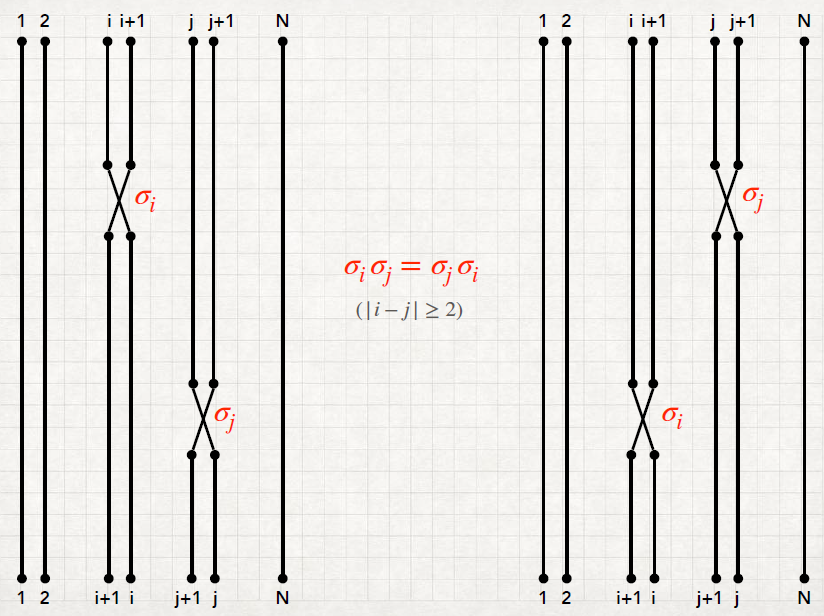
\includegraphics[width=0.95\textwidth]{visual proof 1.png}
    \end{subfigure}
    \begin{subfigure}[b]{0.48\textwidth}
        \centering
        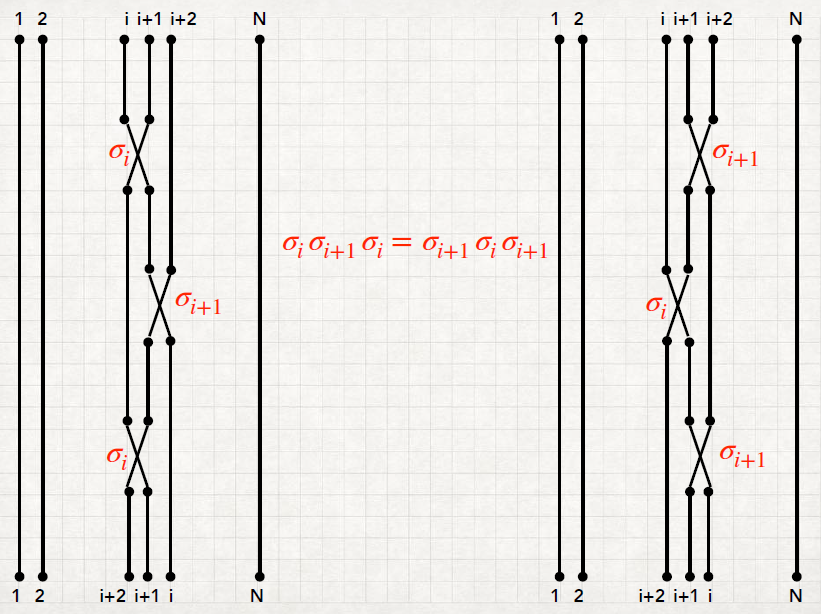
\includegraphics[width=0.95\textwidth]{visual proof 2.png}
    \end{subfigure}
    \caption{Visual proofs of identities between the transpositions}
    \label{fig:visual-proof}
\end{figure}

\subsection{Quantum statistic}
If some objects are indistinguishable, it means that a permutation among those $$\psi(1,2,\dots, N) \xmapsto{\sigma}\psi(\sigma(1), \sigma(2), \sigma(N))$$ doesn't affect the physical content of a wave function, which is $|\psi(x_1, x_2, \dots, x_N)|^2$. That means that the wave function should be the same up to a global phase:
$$\psi(\sigma(1), \sigma(2), \dots,\sigma(N)) = e^{i\phi_\sigma}\psi(1, 2, \dots, N)$$
\gray{Remark: this is a physical property, not a mathematical one.}

If we then decompose a permutation into transpositions that generate it:
$$\sigma = \sigma_{\alpha_1}, \sigma_{\alpha_2}, \dots, \sigma_{\alpha_k} $$
\begin{align*}
    \psi(1,2,\dots, N) \xmapsto{\sigma_{\alpha_1}}&\ \psi(\sigma_{\alpha_1}(1,\dots N)) = e^{i\phi_{\alpha_1}}\ \psi(1,\dots, N) \\
    \xmapsto{\sigma_{\alpha_2}}&\ e^{i\phi_{\alpha_2}} \left(e^{i\phi_{\alpha_1}}\ \psi(1,\dots, N)\right) \\
    \xmapsto{\dots}&\ e^{i(\phi_{\alpha_1} + \phi_{\alpha_2} + \dots + \phi_{\alpha_N})}\ \psi(1,\dots, N) = e^{\phi_\sigma}\psi(1,\dots, N)
\end{align*}
with: $\phi_\sigma = \phi_{\alpha_1} + \phi_{\alpha_2} + \dots + \phi_{\alpha_k}$

Let's now analyze a single transposition: $\sigma_j : \psi(1,\dots, N) \mapsto e^{i\phi_j} \ \psi(1,\dots, N)$, which we will simply write as $\sigma_j \mapsto e^{i\phi_j}$.\\
This must satisfy the (i),(ii),(iii) relations of a transposition and this leads to some considerations on the phase:
\begin{enumerate}[label=\roman*)]
    \item if $|i-j| \ge 2$, then $\sigma_i\sigma_j = \sigma_j\sigma_i$, so:
    \begin{align*}
    \begin{rcases}
        \sigma_i\sigma_j \mapsto e^{i(\phi_i + \phi_j)} \\
        \sigma_j\sigma_i \mapsto e^{i(\phi_j + \phi_i)}
    \end{rcases}
    \iff \phi_i + \phi_j = \phi_j + \phi_i \qquad \text{Trivially satisfied}
    \end{align*}
    
    \item $\sigma_i\sigma_{i+1} \sigma_i = \sigma_{i+1}\sigma_i\sigma_{i+1}$, so:
    \begin{equation*}
    \begin{rcases}    
        \sigma_i\sigma_{i+1}\sigma_i &\mapsto e^{i(\phi_i + \phi_{i+1} + \phi_i)} \\
        \sigma_{i+1}\sigma_i\sigma_{i+1} &\mapsto e^{i(\phi_{i+1} + \phi_i + \phi_{i+1})}
    \end{rcases}
    \iff \phi_i + \phi_{i+1} + \phi_i = \phi_{i+1} + \phi_i + \phi_{i+1}
    \iff \boxed{\phi_i = \phi_{i+1}} \ \forall i
    \end{equation*}
    So $\phi_j = \phi \ \forall j$ and the single transposition $\sigma_j \mapsto e^{i\phi_j}$ becomes simply: $\sigma_j \mapsto e^{i\phi}$

    \item $(\sigma_j)^2 = \id$, so:
    \begin{align*}
        \begin{rcases}
            (\sigma_j)^2 &\mapsto e^{i(\phi + \phi)} = e^{i2\phi} \\
            \quad \id &\mapsto e^{i2\pi n}
        \end{rcases}
        \iff 2\phi = 2\pi n \quad n\in \mathbb{Z}
    \end{align*}
\end{enumerate}

So there are only 2 possibilities (since $\phi \in [0,2\pi[$): 
\begin{align*}
    1. \quad \phi = 0 \qquad &\psi(1,\dots,N) \xmapsto{\sigma_j} \psi(1,\dots,N) \\
    2. \quad \phi = \pi \qquad &\psi(1,\dots,N) \xmapsto{\sigma_j} -\psi(1,\dots,N) \qquad \small{(e^{i\pi} = -1)}
\end{align*}

This applies for a single transposition. For the whole permutation $\sigma = \sigma_{\alpha_1}\sigma_{\alpha_2}\dots\sigma_{\alpha_k}$ and $\phi_\sigma = \phi_{\alpha_1} + \phi_{\alpha_2} + \dots + \phi_{\alpha_k}$. So we have:

\begin{align*}
    1. \quad \phi_{\alpha_j} = 0\quad &\phi_\sigma = 0 \qquad \psi(1,\dots, N) \xmapsto{\forall\sigma \ \in \ \proj_N} \psi(1,\dots,N) &\text{(Bosons)}\\
    2. \quad \phi_{\alpha_j} = \pi \quad &\phi_\sigma = k\pi \qquad e^{i\phi_\sigma} = e^{ik\pi} = (-1)^k \qquad \begin{array}{l} \text{$k$ even } \psi \mapsto\psi \\ \text{$k$ odd } \psi \mapsto -\psi \end{array} &\text{(Fermions)}
\end{align*}

For bosons, the way function is completely symmetric. For fermions it is completely anti-symmetric. \gray{Remark: what we call \textit{bosons} and \textit{fermions} are just due to the statistic and has nothing to do with spin. Only in relativistic quantum mechanics one can prove the spin-statistic theorem.}


\vspace{20pt}
\notedate{(VIII) MON 14/11/2022}
\underline{\textbf{An example: System of N=2 particles in $\R^3$}}\\
We can describe two particles in $\R^3$ with two vectors: $\vec x_1, \vec x_2 \in \R^3$.\\
The Hilbert spaces respectively for a single particle and for two particles are 
\begin{align*}
    \hil_{N=1} = L^2(\R^3) = \{\psi(\vec x_1)\quad \text{square integral}\} \qquad\\
    \hil_{N=2} = L^2(\R^6) = \{\psi(\vec x_1, \vec x_2), \quad \text{square integral}\}
\end{align*}
where $L^2(\R^6) = L^2(\R^3) \circ L^2(\R^3)$.\\
Permutations are described by the permutation group: $\proj_2 = \{\id, \sigma\}$ \quad with $\sigma : x_1 \lrarr x_2$\\
According to our rules, the wave function should be symmetric in the bosonic case and anti-symmetric in the fermionic case. So we define two operators:
\begin{itemize}
    \item Symmetrizer: $\widehat S: \psi(x_1,x_2) \mapsto \frac{\psi(x_1,x_2) + \psi(x_2, x_1)}2 = \psi_+(x_1,x_2) \qquad \text{(symmetric by construction)}$
    \item Antisymmetrizer: $\widehat A : \psi(x_1,x_2) \mapsto \frac{\psi(x_1,x_2) - \psi(x_2, x_1)}2 = \psi_-(x_1,x_2) \qquad \text{(antysimmetric)}$
\end{itemize}

It is easy to show \gray{(as an exercises)}, that $\widehat S$ and $\widehat A$ are projection operators. In fact $\widehat S^\dag = \widehat S \qquad \widehat S^2 = \widehat S \qquad \widehat A^\dag = \widehat A \qquad \widehat A ^2 = \widehat A$\\
If we call $\hil_S$ and $\hil_A$ respectively the spaces of symmetric and anti-symmetric wave functions: $\widehat S : \hil \mapsto \hil_S \qquad \widehat A: \hil \mapsto \hil_A \qquad \hil_S, \hil_A \subset \hil = L^2(\R^6)$

Also: $\widehat S \widehat A = \widehat A \widehat S = 0 \rightarrow \hil_S \perp \hil_A$\\
In fact: 
\begin{align*}
    \braket{\psi_+}{\phi_-} \stackrel{\text{def. of scalar prod.}}{=} &\int d^3 \vec x_1 d^3 \vec x_2 \ \psi^*_+ (x_1,x_2) \phi_-(x_1,x_2) \\
    =\qquad \quad  &\int symm \cdot antisymm = \int \text{anti-symmetric function} = 0
\end{align*}
So we can write $\hil = \hil_S \oplus_\perp \hil_A$. \ In fact every function can be written as the sum of a symmetric and an anti-symmetric function:
$$ \psi(x_1, x_2) = \frac{\psi_+(x_1, x_2) + \psi_-(x_1,x_2)}2$$

Notice that since fermions are described by an anti-symmetric wave function, they can't occupy the same state (Pauli exclusion principle is automatically included in this construction):
$$u_\alpha(x_1) u_\beta(x_2) \mapsto \frac{u_\alpha(x_1) u_\beta(x_2) - u_\alpha(x_1) u_\beta(x_2)}2  = 0 \quad \text{if } \alpha = \beta$$

\vspace{10pt}
\underline{\textbf{Generic $N>2$ particles in $\R^3$}}\\
With $N$ particles, we can have more transpositions. Let's indicate with $P \in \proj_N$ a permutation: $\widehat P : \psi(x_1,x_2,\dots,x_n) \mapsto \psi\left(x_{P^{-1}_{(1)}}, x_{P^{-1}_{(2)}}, \dots, x_{P^{-1}_{(N)}}\right)$. This just re-shuffle the order of particles.\\
We define: 
\begin{align*}
    \widehat S = \frac1{N!} \sum_{P\in\proj_N} \widehat P \qquad &\widehat S : \psi(x_1,x_2,\dots,x_N) \mapsto \frac1{N!} \sum_P \widehat P_\psi \\
    \widehat A = \frac1{N!} \sum_{P\in\proj_N} sgn(P) \widehat P \qquad & sgn(P) = \begin{cases}
        +1 & \text{$P$ is an even permutation} \\
        -1 & \text{$P$ is an odd permutation}
    \end{cases}
\end{align*}

As before, $\widehat S$ and $\widehat A$ are orthogonal projector operators:\\
$\widehat S^\dag = \widehat S \qquad \widehat S^2 = \widehat S \qquad \widehat A^\dag = \widehat A \qquad \widehat A^2 = \widehat A$. \qquad and: $\widehat S\widehat A = \widehat A\widehat S = 0$\\
Also: $\widehat S : \hil_N \to \hil_S \qquad \widehat A : \hil_N \to \hil_A \qquad \hil_S \perp \hil A $\\
$$\implies \hil_N = \underbrace{\hil_S}_{\text{bosons}} \oplus_\perp \underbrace{\hil_A}_{\text{fermions}} \oplus_\perp \underbrace{\hil'}_{\text{non-physical}} $$
with 3 or more particles there are function that ar neither symmetric nor anti-symmetric.\\

We can have an example of $\hil'$ in a system of $N$ particles in $\R^d$. A single particle is described by $\hil_1 = L^2(\R^d)$ with the orthonormal basis: $\{ u_\alpha(x)\}_{\alpha = 1}^\infty$.\\
$N$ particles are described by $\hil_N = \underbrace{L^2(\R^d) \otimes \dots \otimes L^2(\R^d)}_{\text{$N$ times}}$ with the o.n basis\\ 
$\left\{ \psi_{\alpha_1\alpha_2\dots \alpha_N}(x_1,x_2,\dots,x_N) = u_{\alpha_1}(x_1) u_{\alpha_2}(x_2)\dots u_{\alpha_N}(x_N) \right\}_{\alpha_1\alpha_2\dots\alpha_N}$ \\
\gray{Notice that the order is important, because it indicates that there is particle 1 in $\alpha$, particle 2 in $\beta$ etc..}

We aim at describing in an intrinsic way each $\hil_N^{(\widehat S)}, \hil_N^{(\widehat A)}$.
We can define the symmetrizer and antisymmetrizer as:
\begin{align*}
    \widehat S : \psi_{\alpha_1\alpha_2\dots\alpha_N}(x_1,x_2,\dots,x_N) = \psi_{n_1,n_2,\dots, n_k \dots}^{\widehat S} (x_1, x_2, \dots, x_N) \\
    \widehat A : \psi_{\alpha_1\alpha_2\dots\alpha_N}(x_1,x_2,\dots,x_N) = \psi_{n_1,n_2,\dots, n_k \dots}^{\widehat A} (x_1, x_2, \dots, x_N) \\
\end{align*}
Here we can see that the order is no longer important and what matters is just how many particle are in each state. $n_k$ is called \textit{occupation number} and counts just that: how many particles are in the $k$ state. Notice that for bosons there are no constraints ($n_k = 0,1,2,\dots)$, while for fermions there can only be 1 particle at maximum for each state ($n_k = 0,1$).\\
Also, the total number of particles should be constant, so $\boxed{\sum_{k=1}^\infty n_k = N}$\\


    For example, with $N = 3$ we have: $u_\alpha(x_1) u_\beta(x_2) u_\gamma(x_3)$ as the o.n basis and the possible permutations are: 
    $$\begin{matrix}
        1 \ 2 \ 3 & + \\
        1 \ 3 \ 2 & - \\
        2 \ 1 \ 3 & - \\
        2 \ 3 \ 1 & + \\
        3 \ 1 \ 2 & + \\
        3 \ 2 \ 1 & -
    \end{matrix} \qquad \text{(the sign indicate if it's an even or odd permutation)}$$
    
    So we have: 
    \begin{align*}
        \widehat S\left(u_\alpha(x_1) u_\beta(x_2) u_\gamma(x_3)\right) = \frac1{3!} \bigg\{&u_\alpha(x_1) u_\beta(x_2) u_\gamma(x_3) \\
        \pm\  &u_\alpha(x_1) u_\beta(x_3) u_\gamma(x_2)\\
        \pm\ &u_\alpha(x_2) u_\beta(x_1) u_\gamma(x_3)\\
        +\ &u_\alpha(x_2) u_\beta(x_3) u_\gamma(x_1)\\
        +\ &u_\alpha(x_3) u_\beta(x_1) u_\gamma(x_2)\\
        \pm\ &u_\alpha(x_3) u_\beta(x_2) u_\gamma(x_1)  \bigg\}
    \end{align*}
    (and similar for $\widehat A$)
    
    Bosons are described by taking all the signs above (all +), fermions are described by the bottom one (so + - - + + -). However, one could take another combination of plus an minus, obtaining something non-physical ($\in \hil'$)


\section{Second quantization}
We can't work with a wave function spit in $N!$ peaces (in a gas $N\sim 10^{23}$). So, we see the \textit{second quantization}, an algebraic and abstract approach that will lead to very powerful results.

\gray{The approach is different from what it is followed in QFT}

\begin{tikzpicture}
    \node[label=above: classical mechanics (finite dof)] (0) at (4,9) {};
    \node[label=below: classical field theory] (1) at (0,5) {};
    \node[label=below: quantum mechanics] (2) at (8,5) {};
    \node[label=below: QFT] (3) at (4,0) {};
    
    \draw[->](4,9) -- (0,5) node[midway,above left] {$dof \to \infty$};
    \draw[->](4,9) -- (8,5) node[midway,above right] {quantize};
    \draw[->](0,4) -- (4,0) node[midway,below left] {quantize};
    \draw[->](8,4) -- (4,0) node[midway,below right] {$dof \to \infty$};
\end{tikzpicture}

\gray{We follow the right path. Also, we are not interested on time: time is fixed and independent.}

\subsection{Creation/Annihilation operators}
There are two kinds of these operators: bosonic and fermionic
\begin{itemize}
    \item \textbf{Bosonic creation/annihilation operators}
    
    We define $a, a^\dag$ such that $\left[a, a^\dag\right] = aa^\dag - a^\dag a = \id$ on some $\hil$ whose dim$=\infty$\\
    \gray{If that wasn't the case (and $\dim \hil = n$) then $Tr \left[\left[a,a^\dag\right]\right] = Tr\left[\id\right] = n$ But also: \\
    $Tr\left[aa^\dag - a^\dag a\right] = Tr\left[aa^\dag\right] - Tr\left[a^\dag a \right] \stackrel{\text{Tr is circular}}{=} Tr\left[aa^\dag\right] - Tr\left[aa^\dag\right] = 0$\\
    So $\dim\hil = \infty$.}\\
    Notice that they are not self-adjoint operators, so they aren't observables.

    We also define $\widehat N = a^\dag a \qquad \left[\widehat N, a \right] = -a \qquad \left[\widehat N, a^\dag\right] = a^\dag$
    
    For instance, this is the operator used in the 1D harmonic oscillator problem:
    \begin{align*}
    \widehat H &= \frac{\hbar\omega}2 \left(\hat x^2 + \hat p^2\right) &a = \frac{\hat x + i \hat p}{\sqrt 2} \quad a^\dag = \frac{\hat x - i \hat p}{\sqrt2} \\
    &= \hbar \omega \left(a^\dag a + \frac 12\right) &\hat x = \frac{a+a^\dag}{\sqrt2} \quad i\hat p = \frac{a- a^\dag}{\sqrt2} \\
    &= \hbar \omega \left(\widehat N + \frac 12\right)
    \end{align*}

    The o.n basis is given by:
    $$ \widehat H \ket n = \hbar \omega \left(n + \frac12\right) \ket n$$
    
    We won't prove it (it's just algebra), but 
    $$\widehat N \ket n = n\ket n  \qquad \text{when} \quad \ket n = \frac1{\sqrt{n!}}\left(a^\dag\right)^n \ket 0 \qquad \widehat N \ket 0 = 0 \quad \text{(g.s. or vacuum state)}$$

    $\widehat N$ is called number operator, because the eigenvalue is just the number of quanta. The base $\left\{\ket n\right\}_{n=0}^\infty$ is called \textbf{Fock basis} and it is an o.n. basis on $\hil$.\\
    \gray{Of course, one can chose another base, but we know very well how this base here behaves.}\\
    Applying the creation/annihilation operators just consists in going up or down in the ladder in Fig. \ref{fig:creation-annihilation}:
    \begin{align*}
        &a\ket n = \sqrt{n-1}\ket{n-1} \quad &\text{Going down the ladder (destroying a particle)}\\
        &a^\dag \ket n = \sqrt n \ket{n+1} \quad &\text{Going up the ladder(creating a particle)}
    \end{align*}

    \begin{figure}[ht]
        \centering
        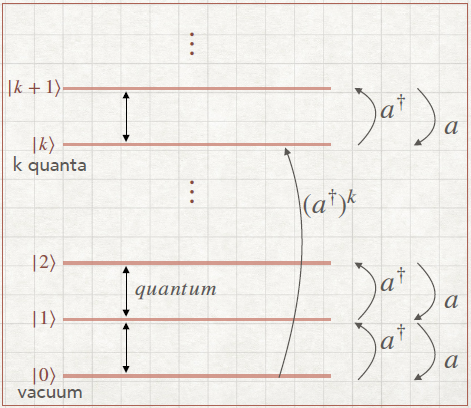
\includegraphics[width = 7cm]{creation-annihilation.png}
        \caption{Creation/annihilation "ladder" for bosons.}
        \label{fig:creation-annihilation}
    \end{figure}
    
    \gray{Also, the fact that we can apply $a^\dag$ many times is another reason why the Hilbert space should have $\dim = \infty$.}

    \item \textbf{Fermionic creation/annihilation operators}

    We define $c, c^\dag$ such that $\left\{c,c^\dag\right\} = cc^\dag + c^\dag c = \id $ and $ c^2 = \left(c^\dag\right)^2 = 0$. \\
    As before we also define the number operator \\
    $\widehat N = c^\dag c \qquad \left[\widehat N, c \right] = -c \qquad \left[\widehat N, c^\dag\right] = c^\dag$ \\

    For instance, this is the operator used in a spin $1/2$ particle system. Given the Pauli matrices:
    $$ \sigma^x = \frac 12\begin{bmatrix} 0 & 1 \\ 1& 0 \end{bmatrix} \qquad
    \sigma^y = \frac 12\begin{bmatrix} 0 & -i \\ i& 0 \end{bmatrix} \qquad
    \sigma^z = \frac 12\begin{bmatrix} 1 & 0 \\ 0 & -1 \end{bmatrix} $$
    satisfying $\left[\sigma^\alpha, \sigma^\beta\right] = \epsilon_{\alpha\beta\gamma}\sigma^\gamma$ , \qquad one can construct:
    $$\sigma^{\pm} \equiv \sigma ^x \pm i \sigma ^y \implies 
    \sigma^+ = \begin{pmatrix}0&1\\0&0\end{pmatrix} \quad
    \sigma^- = \begin{pmatrix}0&0\\1&0\end{pmatrix}$$
    such that \qquad $ \left\{\sigma^-, \sigma^+\right\} = \id_{2\times2} \qquad \left(\sigma^-\right)^\dag = \sigma^+ \qquad \left(\sigma^-\right)^2 = \left(\sigma^+\right)^2 = 0$
    
    The Fock basis is the o.n. basis given by: \\
    $\ket 0 \text{ vacuum} \qquad \ket 1 = c^\dag \ket 0 \qquad \ket 2 = c^\dag c^\dag \ket 0 = 0 $ \quad (since $\left(c^\dag\right)^2 = 0$)
    
    So we have only two possible states: $\widehat N \ket 0 = 0 \qquad \widehat N \ket 1 = 1\cdot \ket 1$\\ as shown in Fig. \ref{fig:creation-annihilation(fermions)}.

    \begin{figure}[h]
        \centering
        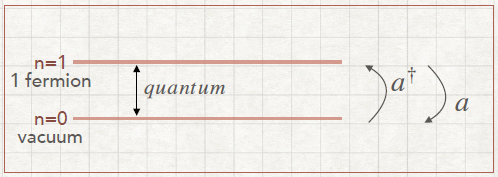
\includegraphics[width = 7cm]{creation-annihilation(fermions).png}
        \caption{Creation/annihilation "ladder" for fermions.}
        \label{fig:creation-annihilation(fermions)}
    \end{figure}

    As before $\widehat N\ket n = n\ket n$ is called number operator, but this time $n = 0,1$
\end{itemize}
In both cases the vacuum $\ket 0 (n =0)$ is the lowest level and it's defined by $a\ket 0= 0\quad  c \ket 0 = 0$

\notedate{17/11/2022}
From now on we will indicate with $a,a^\dag$ both the fermionic and bosonic operators and we will write: $\left[a,a^\dag\right]_{\mp} = \left. aa^\dag \mp a^\dag a\right|_F^B$

\subsection{Fock Space}

We will give now a rather simple algebraic construction of the Fock space $\fock_F$, showing that it has all the required properties.

We want to construct $\hil^{(S/A)} \equiv \bigoplus_{N=0}^\infty \hil_N^{(S/A)}$ in an intrinsic way.\\
For each element of an (arbitrary) o.n. basis $\left\{u_\alpha(x)\right\} \in L^2(\R^3)$ in a single particle $\hil$, we can consider a couple of creation/annihilation operators $a_\alpha^\dag, a_\alpha$ such that:
$$ \left[a_\alpha, a_\beta \right]_\mp = \left[a^\dag_\alpha, a_\beta ^\dag\right]_\mp = 0 \quad \forall \alpha, \beta \qquad \left[a_\alpha, a_\beta^\dag\right]_\mp = \delta_{\alpha\beta}$$
\gray{The $\alpha$'s are the quantum number labeling the one-particle basis $\{u_\alpha\}$.}\\
These are called \textit{canonical commutation relations (CRR)}. Note that this relations imply automatically that $(a_\alpha)^2 = (a_\alpha^\dag)^2 = 0$. In this case:
\begin{enumerate}[label=\roman*.]
    \item We can define the vacuum state $\ket 0$ by requiring that the $a_\alpha$'s annihilate it:
    $$\ket 0 :\quad a_\alpha \ket 0 = 0 \quad  \forall \alpha$$
    We will see immediately that this single requirement allows for a complete construction of the Fock space. \gray{In fact we can construct\\ $\hil_0^{B/F} = \left\{\lambda \ket 0, \ \lambda \in \Complex\right\} \stackrel{\text{isomorphic to}}\simeq \Complex$}

    \item What happens if the creation operator is applied to $\ket 0$?\\
    $a^\dag_\alpha\ket 0 \iff u_\alpha(x)$ creates one particle in the state $\alpha$. The one-particle state will be defined as:
    $$a^\dag_\alpha\ket 0 = \ket{0,\dots, 0, 1_\alpha, 0,\dots}$$
    \gray{For example:
    $$\hil_1^{B/F} = \left\{\left\{a_\alpha^\dag\ket 0\right\}_{\alpha=1}^\infty \text{o.n basis}\right\} \simeq L^2(\R^3)$$
    $$\sum_{\alpha=1}^\infty f_\alpha a_\alpha^\dag \ket 0 \iff \ket{f(x)} = \sum_\alpha f_\alpha u_\alpha(x) $$}

    \item Then, recursively, what about $N=2$?\\
    We'll start with one particle in the state $\alpha$ ($a_\alpha^\dag\ket 0$), then we'll add the second one:
    \begin{itemize}
        \item First case: second particle in $\alpha$\\
        For Bosons: $\left(a^\dag\right)^2 \ket 0$ \qquad (2 particles in $\alpha$)\\
        For Fermions: $\left(a^\dag\right)^2 \ket 0 = 0$ \qquad (The rules of our creation/annihilation algebra implicitly define Pauli exclusion principle)
        \item Second case: second particle in $\beta \ne \alpha$\\
        Both for bosons and fermions we have: $a_\beta^\dag a_\alpha^\dag \ket 0$\\
        \gray{What if instead $a_\alpha^\dag a_\beta^\dag \ket 0$ (we add first the particle in $\beta$ and the the one in $\alpha$) ? From the condition on the (anti)commutator, we have that $a_\alpha^\dag a_\beta^\dag\ket0 = \pm a_\beta^\dag a_\alpha ^\dag\ket 0$.}
    \end{itemize}

    \item We can now generalize to $N$ particles:
    \begin{align}
        \ket{n_1,n_2,\dots,n_k,\dots} \equiv& \ \eta \  \sqrt{\frac1{\prod_j n_j!}}\left(a_1^\dag\right)^{n_1}\left(a_2^\dag\right)^{n_2} \dots \left(a_k^\dag\right)^{n_k} \dots \ket 0 \iff \label{eq:Nparticles}\\
        \xLeftrightarrow{\text{1-1 corresp.}}\ &  \psi_{\{k\}} =\  ^{\hat S}_{\hat A}\left(u_{\alpha_1}(x_1), \dots, u_{\alpha_k}(x_k)\right) \quad \text {o.n. basis for $\hil_S, \hil_A$} \nonumber
    \end{align}
    where $\eta = \begin{cases} 1 &\text{for bosons} \\ (-1)^{\sum_{j=1}^{k-1} n_j} &\text{for fermions}\end{cases}$\\
    since we pick up a -sign every time we commute to bring $a_k^\dag$ to $\ket{n_k}$.\\
    Remember also that $n_j$ indicate the number of particles in the state $j$.
    
    Then if we chose $\ket{n_1,\dots,n_k\dots}$ as an o.n basis, we can define $\hil^{B/F}$ "automatically" from $a^\dag$:
    $$ \hil^{S/A} = \hil^{B/F} = \left\{\left\{ \ket{n_1,\dots,n_k\dots}\right\} \text{o.n. basis}\right\}$$        
\end{enumerate}

\begin{itemize}
    \item For example, let's analyze two 1-particle states $\alpha \ne \beta$.\\
    $a_\alpha^\dag\ket 0 \lrarr u_\alpha \qquad a_\beta^\dag \ket 0 \lrarr u_\beta \qquad \qquad \left(a_\beta^\dag\ket 0 \right)^\dag = \bra 0 a_\beta$ \qquad \qquad Then: 
    \begin{align*}
    \braket{u_\beta}{u_\alpha} \iff &\brakett{0}{a_\beta a_\alpha^\dag}{0} = 0 &\text{since $a_\alpha a_\beta^\dag \mp a_\beta^\dag a_\alpha = 0$}\\
    & \brakett0 {\pm a_\alpha^\dag a_\beta}0 = 0 &\text{since $a_\beta\ket 0 = 0$}
    \end{align*}
    
    \gray{The trick is to put all the annihilation operators to the right (not only in this case, but always).}
\end{itemize}
Now let's analyze better for $N$ particles: we expect $a_k^\dag \ket{n_1 \dots n_k \dots}$ to be proportional to $\ket{n_1 \dots (n_k+1) \dots} $
$$\ket{n_1 \dots (n_k+1) \dots } \stackrel{(\ref{eq:Nparticles})}= \frac\eta{\sqrt{\prod_{i\ne k} n_i!(n_k+1)!}} \left(a_1^\dag\right)^{n_1}\dots\left(a_k^\dag\right)^{n_k+1}\dots \ket 0$$
If we compute:
$$ a_k^\dag \frac1{\sqrt{\prod_i n_i!}} \left(a_1^\dag\right)^{n_1}\left(a_2^\dag\right)^{n_2}\dots \left(a_k^\dag\right)^{n_k}\dots \ket 0 = \sqrt{n_k+1} \ \eta \ \ket{n_1,n_2, \dots, (n_k+1), \dots}$$

Therefore \qquad $a_k^\dag : \hil_N^{B/F} \to \hil_{N+1}^{B/F}$

\gray{One can prove (as an exercise) that $a_k\ket{n_1\dots n_k} = \eta \sqrt{n_k} \ket{n_1,\dots, (n_k-1),\dots}$\\
and if $n_k= 0 \implies a_k\ket{n_i\dots n_k} = 0$ \quad so that \qquad $a_k: \hil_N^{B/F} \to \hil_{N-1}^{B/F}$}\\

We can thus construct the \textbf{Fock space} (useful in the grancanonical):
$$\hil_F^{B/F} = \bigoplus_{N=0}^\infty \hil_N^{B/F}$$

It is also useful to define the operator $\hat n_k$ which counts how many particles occupy the k-th state: $\hat n_k \equiv a_k^\dag a_k$
$$\hat n_k: \hil_N^{B/F} \to \hil_N^{B/F} \qquad \hat n_k \ket{n_1\dots n_k\dots} = n_k \ket{n_1 \dots n_k\dots}$$
the so-called \textit{Fock basis}: $\left\{\ket{n_1 \dots n_k\dots}\right\}_{\left\{n_1,n_2\dots\right\}}$ is a basis of eigenstates for $\hat n_k$\\
and we can build the number operator $\widehat N$, that counts the total number of particles $\widehat N = \sum_{k=1}^\infty \hat n_k$.\\

What we have seen is the following:\\
\Th \begin{enumerate}
    \item The multi-particle states are an o.n basis for $\hil_N^{S/A}$ (in both cases):
    $$\braket{n_1',n_2', \dots, n_k' \dots}{n_1,n_2,\dots, n_k\dots} = \delta_{n_1'n_1}\delta_{n_2'n_2}\dots \delta_{n_k'n_k} \dots$$
    
    \item annihilation: \qquad $ a_k : \hil_N^{S/A} \to \hil_{N-1}^{S/A}$
    $$ a_k\ket{n_1,n_2, \dots n_k\dots} = \eta \ \sqrt{n_k} \ket{n_1, n_2, \dots , (n_k-1) \dots}$$
    where $\eta = \begin{cases} 1 &\text{for bosons} \\ (-1)^{\sum_{j=1}^{k-1} n_j} &\text{for fermions}\end{cases}$\\
    
    \item creation: \qquad $a_k^\dag : \hil_N^{S/A} \to \hil_{N+1}^{S/A}$
    $$ a_k^\dag\ket{n_1,n_2, \dots n_k\dots} = \sqrt{n_k+1} \ket{n_1, n_2, \dots , (n_k+1) \dots}$$
    Note that in the fermionic case we have $a_k^\dag \ket {n_1,n_2, \dots, n_k, \dots} = 0$ if $n_k = 1$. This is again the expression of Pauli exclusion principle.

    \item the operator $\hat n_k = a_k^\dag a_k$ counts how many particles occupy the k-th state:
    $$\hat n_k \ket{n_1,n_2,\dots, n_k,\dots} = n_k \ket{n_1,n_2, \dots, n_k, \dots}$$
    and the operator $\widehat N = \sum_k \hat n_k = \sum_k a_k^\dag a_k$ counts the total number of particles:
    $$ \widehat N\ket{n_1,n_2, \dots n_k\dots} = \left(\sum_k n_k = N\right) \ket{n_1,n_2, \dots n_k\dots}$$
\end{enumerate}

\underline{Remarks:}
\begin{itemize}
    \item The states $\ket{n_1,n_2, \dots, n_k}$, hence any state in $\hil_N^{(S/A)}$, are symmetric/antisymmetric by construction, thanks to the commutation/anticommutation relations among the creation/annihilation operators.
    \item As we've seen, in the fermionic case Pauli exclusion principle is automatically encoded.
    \item States are written in terms of creation/annihilation operators: in particular, single particle states $\ket{e_n}$ are in 1-1 correspondence with $a_n^\dag\ket0$. In general, a generic single-particle state $\ket f = \sum_n f_n\ket e_n \quad \text{with } f_n = \braket{e_n}{f}$ is represented by the vector in the Fock space: $\sum_n f_n a_n^\dag \ket 0 \equiv \psi^\dag (f)\ket 0$.\\
    So we say that a state $\ket f$ is represented by/becomes the operator $\psi^\dag (f)$\\
    This is called the \textit{second quantization procedure}.
\end{itemize}

\begin{comment}
Let's consider $\psi_{S,A} (x_1, x_2, \dots x_N) \in \left(L^2\left(\R^3\right)\right)_{B/F}^{\oplus N}$. We can write the Hamiltonian:
$$ \widehat H_N = \underbrace{\sum_{j=1}^N \frac{\widehat{\vec{p_j}}}{2m} + \sum_{j= 1}^N V_{ext}\left(\hat x_k)\right)}_{\sum_{j=1}^N \widehat O^{(1)} \left(\hat x_j\hat p_j,\right) \text{ one particle operator}} + \underbrace{\sum_{i<j} V_{int} \left(\hat x_i, \hat x_j\right)}_{\text{2 particle operators}}$$
\end{comment}

\subsection{Field operator}
The creation and annihilation operators introduced so far are tied to the (arbitrary, of course) choice of a basis of one-particle states. The state $a_\alpha^\dag\ket 0$ corresponds then to the creation of one particle in the state $u_\alpha$ out of the vacuum or, more generally, $a_\alpha^\dag \ket {n_1,\dots, n_i,\dots}$ will correspond to the addition of a particle in the same state. What if we want to “create” an additional particle in an arbitrary state represented by the wavefunction $f(\vec x) = \sum_\alpha u_\alpha(\vec x) \braket{u_\alpha}f$?\\
A little thought suffices to conclude that, if $a_\alpha^\dag$ creates a particle in the basis state $u_\alpha$, then a particle in a generic state $f \in L^2(\R^d)$ will be created by the operator: 
\begin{equation}\label{eq:creation}
    \psi^\dag(f) = \sum_\alpha \braket{u_\alpha}f a_\alpha^\dag
\end{equation}
And the adjoint of $\psi^\dag(f)$:  
\begin{equation}\label{eq:annihilation}
    \psi(f) = \sum_\alpha \braket f{u_\alpha} a_\alpha    
\end{equation}
will act as the corresponding annihilation operator.

Let's make things a little more formally: firstly, we chose to work within the coordinate representation:\\
$$\hil = L^2(\R^d) \qquad \{\ket{e_\alpha} = u_\alpha\}_\alpha \qquad f(x) = \sum_\alpha u_\alpha(x) f_\alpha \quad f_\alpha = \int_{\R^d} u^*_\alpha(x) f(x) = \braket{u_\alpha} f$$
Then, if the associated creation/annihilation operators are denoted with $a_\alpha,a_\alpha^\dag$, we define the creation/annihilation \textbf{field operators} as:
$$\psi^\dag(x) = \sum_\alpha u_\alpha^*(x)a_\alpha^\dag \qquad \psi(x) = \sum_\alpha u_\alpha(x) a_\alpha$$
and the (\ref{eq:creation}) and (\ref{eq:annihilation}) can be written as integrals of those (see the following theorem).

\gray{It is pretty obvious that $\psi^\dag(\vec x)$ is a rather ill-defined operator on Fock space. Indeed, it is easily checked that, say, $\|\psi^\dag(\vec x)\ket0\|^2 = \delta(\vec 0)$, a diverging quantity, and hence that $\psi^\dag(\vec x) \ket 0$ cannot be considered as a vector in Fock space. $\psi^\dag(\vec x)$ has rather to be considered as a “distribution-valued” operator, i.e. it acquires a reasonable mathematical meaning only when it operates on functions in $L^2(\R^d)$ like in the definition of $\psi^\dag(f)$ below.}\\

\Th \begin{enumerate}[label=\roman*)]
    \item (\ref{eq:creation}) can be expressed by the field operator:
    $$\psi^\dag(f) = \int_{\R^d} \psi^\dag(x) f(x) \qquad \text{in particular: } \psi^\dag(u_\alpha) = \int_{\R^d} \psi^\dag(x)u_\alpha(x) = a_\alpha^\dag$$
    
    \item Some nice commutation relations holds:
    \begin{align*}
        \left[\psi(f) \psi(g)\right]_\mp = \left[\psi^\dag(f) \psi^\dag(g)\right]_\mp = 0& \qquad \left[\psi(f) \psi^\dag(g)\right]_\mp = \angles{f,g}\\
        \left[\psi(x) \psi(y)\right]_\mp = \left[\psi^\dag(x) \psi^\dag(y)\right]_\mp = 0& \qquad \left[\psi(x) \psi^\dag(y)\right]_\mp = \delta(x-y)
    \end{align*}

    \item The field operators are independent on the chosen basis: 
    $$\psi^\dag(x) = \sum_\alpha u^*_\alpha(x) a_\alpha^\dag = \sum_\beta v_\beta^*(x) b_\beta^\dag$$
\end{enumerate}

\Pf \begin{enumerate}
    \item[(i)]
    \begin{align*}
        \int_{\R^d} \psi^\dag(x) f(x) = \int f(x) \sum_\alpha u_\alpha^* a_\alpha^\dag = \sum_\alpha \int \underbrace{f(x)u_\alpha^*}_{\braket fu} a_\alpha^\dag = \sum_\alpha f_\alpha a_\alpha^\dag = \psi^\dag(f)
    \end{align*}
    \item[(ii)]
    \begin{itemize}
        \item $$ \left[\psi(f), \psi(g)\right]_\mp = \left[\sum_\alpha u_\alpha(x) a_\alpha \ , \ \sum_\beta v_\beta(y)a_\beta\right]_\mp = \sum_{\alpha\beta} u_\alpha v_\beta \left[a_\alpha, a_\beta\right]_\mp = 0$$
        \item $\left[\psi^\dag(x), \psi^\dag(y)\right] = 0$ is proven similarly.

        \item \begin{align*} 
            \left[\psi(f), \psi^\dag(g)\right]_\mp &= \left[\sum_\alpha f_\alpha a_\alpha \ , \ \sum_\beta g_\beta^* a_\beta^\dag\right]_\mp = \sum_{\alpha\beta} f_\alpha g_\beta^* \underbrace{\left[a_\alpha, a_\beta^\dag\right]}_{\delta_{\alpha\beta}}\\
            &= \sum_\alpha f_\alpha g_\alpha^* = \angles{f,g} \mathbbm{1}
        \end{align*}

        \item From (i): $ \psi^\dag (f) = \int f(x) \psi^\dag(x) \qquad \psi(g) = \int g^*(y) \psi(y)$
        $$ \angles {f,g} = \int d^dx\int d^dy \ f(x)g^*(y) \left[\psi(y), \psi^\dag(x)\right]_\mp \implies \left[\psi(y), \psi^\dag(x)\right] = \delta_{(x-y)} \mathbbm{1}$$
    \end{itemize}

    \item[(iii)] Let's have another base $\{v_\beta(x)\}$ from which we can get different creation annihilation operators $b_\beta, b_\beta^\dag$.
    \begin{align*}
        \{u_\alpha(x)\} \to a_\alpha,a_\alpha^\dag &\implies \ket{n_1,n_2, \dots, n_k \dots} = C\ \left(a_1^\dag\right)^{n_1}\left(a_2^\dag\right)^{n_2} \dots \ket 0\\
        \{v_\beta(x)\} \to b_\beta,b_\beta^\dag &\implies \ket{m_1,m_2, \dots, m_k \dots} = C\ \left(b_1^\dag\right)^{m_1}\left(b_2^\dag\right)^{m_2} \dots \ket 0 
    \end{align*}
    \begin{align*}
        f(x) = \sum_\alpha f_\alpha u_\alpha(x) \qquad &\psi^\dag(f) = \sum_\alpha f_\alpha a_\alpha^\dag\\
        f(x) = \sum_\beta \tilde f_\beta v_\beta(x) \qquad &\psi^\dag(f) = \sum_\beta f_\beta b_\beta^\dag
    \end{align*}
    We won't prove it, but the expressions on the right are equal. That means that they are independent on the chosen basis.
    
    This is also true for the field operators:
    $$ \psi^\dag(x) = \sum_\alpha u_\alpha^* (x) a_\alpha^\dag = \psi^\dag(x) = \sum_\beta v_\beta^* (x) b_\beta^\dag$$
    The two expressions are the field operator expressed in two different basis. Since they are equal, it means it is basis independent.
\end{enumerate}
\EndPf

\subsection{Observable operators}
\notedate{(IX) MON 21/11/2022}
We want now to characterize how observables act in Fock space.

\underline{\textbf{Single particles observables}}\\
In first quantization, single particles observables are written in $\hil_N^{S/A}$ as:
$$\widehat A: \sum_{j=1}^N A^{(1)} (\vec p_j, \vec x_j)$$
where $A^{(1)}$ is an operator on the single particle $\hil$, and let $\{u_\alpha\}$ be the basis of the eigenfunctions of $A^{(1)}$, i.e.: $A^{(1)} (\vec p, \vec x) u_\alpha(x) = \epsilon_\alpha u_\alpha(x)$\\
A trivial example could be the harmonic oscillator: $\widehat A = \sum_{j=1}^N \underbrace{\left(\frac{\widehat{\vec p_j}^2}{2m} + \frac{\omega^2 m}2 \hat x_j^2\right)}_{A^{(1)}(p_j,x_j)}$

So (in the following, $C$ is a constant that we don't care about):
$$\psi_{n_1,n_2,\dots , n_k\dots}(x_1,x_2,\dots,x_N) = C \ ^{\hat S}_{\hat A}\left(u_{\alpha_1}(x_1)\dots u_{\alpha_N}(x_N)\right)$$
Multiplying both sides by $\widehat A = \sum_{j=1}^N A^{(1)}(\vec p_j, \vec x_j)$:
\begin{align*}
    \widehat A \ \psi_{n_1,n_2,\dots , n_k\dots}(x_1,x_2,\dots,x_N) &= C \ ^{\hat S}_{\hat A}\left(\sum_{j=1}^N A^{(1)} (\vec p_j, \vec x_j)\left( u_{\alpha_1}(x_1)\dots u_{\alpha_N}(x_N)\right)\right) \\
    &= C \ ^{\hat S}_{\hat A}\left(\sum_{j=1}^N \epsilon_{\alpha_j}\right) \left( u_{\alpha_1}(x_1)\dots u_{\alpha_N}(x_N)\right)
    \intertext{using linearity of all the operators:}
    &= \left(\sum_{j=1}^N \epsilon_{\alpha_j}\right) \psi_{n_1,n_2,\dots}(x_1,x_2,\dots,x_N)
    \intertext{Another way to write it could be:}
    &= \left(\epsilon_{\alpha_1} + \epsilon_{\alpha_2} + \dots + \epsilon_{\alpha_N}\right) \psi_{n_1,\dots, n_k, \dots}
    \intertext{and another one:}
    &= \left(\sum_{\alpha=1}^\infty \epsilon_\alpha n_\alpha\right) \psi_{n_1,n_2,\dots}
\end{align*}
What we have shown is that: $\widehat A\psi_{n_1,n_2,\dots}(x_1,\dots,x_N) = \left(\sum_{\alpha=1}^\infty\epsilon_\alpha n_\alpha \right) \psi_{n_1,n_2,\dots}(x_1, \dots, x_N)$\\
We now want to define in the Fock space an operator that acts the same as our original operator, so such that:
$$\widehat A \ket{n_1, n_2 \dots, n_k, \dots} = \left(\sum_\alpha \epsilon_{\alpha_n}n_\alpha\right) \ket{n_1, n_2 \dots, n_k, \dots}$$

It follows that, in Fock space $\fock_N^{B/F}$, the "second-quantized" version of $\widehat A$ is:
\begin{equation}\label{eq:single particle operator}
    \boxed{\widehat A_F = \sum_{\alpha=1}^\infty \epsilon_\alpha \hat n_\alpha = \sum_{\alpha=1}^\infty \epsilon_\alpha a_\alpha^\dag a_\alpha}
\end{equation}
with $\epsilon_\alpha = \brakett{u_\alpha}{A^{(1)}}{u_\alpha}$ \qquad  or equivalently: $A^{(1)} (\vec p, \vec x) u_\alpha(x) = \epsilon_\alpha u_\alpha(x)$\\
\gray{Notice that $\hat n_\alpha = a_\alpha^\dag a_\alpha$, so this operator destroy then create a particle, thus the total number of particle is conserved.}\\

\begin{comment}
What we have done seems to be affected by the chosen basis $\{u_\alpha(x)\}$. But what to do if we don't know the basis? The idea is to choose a base and from that we get creation/annihilation operators $a_\alpha,a_\alpha^\dag$

Let's have another base $\{v_\beta(x)\}$ from which we can get different creation annihilation operators $b_\beta, b_\beta^\dag$.
\begin{align*}
    \{u_\alpha(x)\} \to a_\alpha,a_\alpha^\dag &\implies \ket{n_1,n_2, \dots, n_k \dots} = C\ \left(a_1^\dag\right)^{n_1}\left(a_2^\dag\right)^{n_2} \dots \ket 0\\
    \{v_\beta(x)\} \to b_\beta,b_\beta^\dag &\implies \ket{m_1,m_2, \dots, m_k \dots} = C\ \left(b_1^\dag\right)^{m_1}\left(b_2^\dag\right)^{m_2} \dots \ket 0    
\end{align*}
\begin{align*}
    f(x) = \sum_\alpha f_\alpha u_\alpha(x) \qquad &\psi^\dag(f) = \sum_\alpha f_\alpha a_\alpha^\dag\\
    f(x) = \sum_\beta \tilde f_\beta v_\beta(x) \qquad &\psi^\dag(f) = \sum_\beta f_\beta b_\beta^\dag
\end{align*}
We won't prove it, but the expressions on the right are equal. That means that they are independence on the chosen basis.

This is also true for the field operators:
$$ \psi^\dag(x) = \sum_\alpha u_\alpha^* (x) a_\alpha^\dag = \psi^\dag(x) = \sum_\beta v_\beta^* (x) b_\beta^\dag$$
The two expressions are the field operator expressed in two different basis. Since they are equal, it means in is basis independent.
\end{comment}

We have shown that both the creation operators and the field operator are base-independent. However this is not the case for the single particles observables in Fock space $\widehat A_F$ in eq. (\ref{eq:single particle operator}). In fact, if $\{u_\alpha\}$ is a generic basis and not the basis of eigenfunctions of $A^{(1)}$, we have:
$$ \brakett{u_\beta}{\hat A^{(1)}\left(\vec p, \vec x\right)}{u_\alpha} = \epsilon_\alpha \braket{u_\beta}{u_\alpha} = \epsilon_\alpha \delta_{\alpha\beta}$$
$$ \widehat A_F = \sum_{\alpha \beta} \brakett{u_\beta}{\hat A^{(1)}}{u_\alpha} a_\alpha^\dag a_\beta$$
Which is equal to eq. (\ref{eq:single particle operator}) only if we add $\delta_{\alpha\beta}$. 

Choosing a different basis $v_j$ with the corresponding creation/annihilation operators $b_j,b_j^\dag$:
$$\widehat A_F = \sum_{jk} \underbrace{\brakett{v_j}{\hat A^{(1)}}{v_k}}_{t_{jk}}b_j^\dag b_k  = \sum_{jk} t_{jk} b_j^\dag b_k$$

This operator is no longer diagonal (indexes are different). It destroys a particle in the state $k$ and create another one in the state $j$.\\

Using the definition of the field operators $\psi(\vec x), \psi^\dag(\vec x)$, there also exists a way to write everything without referring to a basis:
$$ \widehat A = \sum_{j=1}^N A^{(1)}\left(\vec p_j, \vec x_j\right) \xrightarrow[]{\text{in Fock space}} \widehat A_F = \int d^3x\  \psi^\dag(x)A^{(1)}\left(\vec p, \vec x\right) \psi(x)$$
In fact: $\psi^\dag(x) \equiv \sum_\alpha u_\alpha^* (x) a_\alpha^\dag \qquad \psi(x) \equiv \sum_\beta u_\beta (x) a_\beta $:
\begin{align*}
    A &= \int d^3 x \left(\sum_\alpha u_\alpha^*(x) a_\alpha^\dag\right) A^{(1)} \left(\sum_\beta u_\beta (x) a_\beta\right) \\
    &= \sum_{\alpha\beta}\underbrace{\int d^3x\ u_\alpha^*(x)A^{(1)}(\vec p, \vec x) u_\beta(x)}_{\brakett{u_\alpha}{A^{(1)}}{u_\beta}} a_\alpha^\dag a_\beta \\
    &= \sum_{\alpha\beta} t_{\alpha\beta} a_\alpha^\dag a_\beta
\end{align*}
Now let's see some examples:
\begin{enumerate}[label=\roman*)]
    \item Density operator\\
    On a single particle $u(x) \in L^2\left(\R^3\right)$, we have:
    $$ \hat \rho^{(1)} = \delta(x-x_0) \qquad \hat \rho^{(1)}: u(x) \mapsto \int_{\R^3} d^3 x u(x) \delta(x-x_0) = u(x_o)$$
    For $N$ particles, we have $N$ coordinates: 
    $$x_1, x_2, \dots x_N \qquad \hat \rho(y) = \sum_{j=1}^N \delta (y-x_j)$$
    In Fock space it becomes:
    $$ \hat \rho_F = \int d^3y\ \psi^\dag(y) \rho^{(1)}\psi(y) = \int d^3y\ \psi^\dag (y) \delta(y-x) \psi(y) = \psi^\dag(x) \psi(x)$$

    \item Number operator\\
    The previous operator is called density operator because the number operator is expressed by: $ \hat N = \int_{\R^3} d^3 x \hat\rho (x)$. In fact, in Fock space the number operator is:
    \begin{align*}
        \hat N_F &= \int d^3x\ \psi^\dag(x) \psi(x) &\text{using definition of $\psi^\dag, \psi$}\\
        &= \int d^3 x\left(\sum_\alpha u_\alpha^*(x) a_\alpha^\dag\right) \left(\sum_\beta u_\beta(x) a_\beta\right) \\
        &= \sum_{\alpha\beta}\underbrace{\left(\int d^3 x u_\alpha^*(x) u_\beta(x) \right)}_{\braket {u\alpha}{u_\beta} = \delta_{\alpha\beta}} a_\alpha^\dag a_\beta = \sum_\alpha a_\alpha^\dag a_\alpha = \sum_\alpha \hat n_\alpha
    \end{align*}
    which is just the total number of particle.

    \item Free hamiltonian\\
    With $N$ particles the hamiltonian is $$ H = \sum_{j=1}^N \underbrace{\frac{\vec {p_j}^2}{2m}}_{A^{(1)}(\vec p_j, x_j)}$$
    acting in $L^2(\R^3) = \phi(x_1,x_2 \dots, x_N)$

    Using the substitution: $\vec p \mapsto -i\hbar\nabla$
    $$\frac{\vec {p_j}^2}{2m}\phi(x_1, \dots, x_N) = \frac{\left(-i\hbar\nabla_{x_j}\right)^2}{2m} \phi(x_1,\dots, x_j \dots x_N)$$
    with $A^{(1)}(\vec p_j, x_j) = \frac {\hbar^2}{2m} \nabla_x^2$.

    In Fock space the hamiltonian becomes:
    \begin{equation}\label{eq:hamiltonian fock}
        H_F = \int d^3x\ \psi^\dag (x) A^{(1)}(\vec p_j, x_j)\psi(x) = \int d^3x\ \psi^\dag(x) \left[\frac{\hbar^2}{2m} \nabla^2_x\right]\psi(x)
    \end{equation}

    \begin{equation}\label{eq:nabla squared}
        \nabla^2_x \psi(x) = \nabla^2_x\left(\sum_\alpha u_\alpha(x) a_\alpha\right) = \sum_\alpha \left(\nabla^2_x u_\alpha(x)\right) a_\alpha    
    \end{equation}
    
    We want to choose $u_\alpha(x)$ such that $\nabla^2_x u_\alpha(x) = \epsilon_\alpha u_\alpha(x)$ \\
    where $\alpha = \vec k$ ($\alpha$ is the momentum).\\
    The solution is to choose the single particle o.n. basis: $u_{\vec k} = e^{i\vec k \cdot\vec x}$\gray{$/\sqrt V$}. \gray{We will comment later about the normalization factor $1/\sqrt V$}\\
    In fact:
    $$ \nabla^2_x u_{\vec k}(x) = \underbrace{-{\vec k}^2}_{\epsilon_{\vec k}} u_\alpha(x) \implies (\ref{eq:nabla squared}) = \sum_{\vec k} (-k)^2 u_{\vec k}(x) a_{\vec k}$$
    And the hamiltonian in Fock space (\ref{eq:hamiltonian fock}) becomes:
    \begin{align*}
        H_F &= \int d^3x\ \psi^\dag(x) \left(-\frac{\hbar^2}{2m}\nabla^2_x\right) \psi(x)\\
        &= \int d^3x \left(\sum_{\vec k'} u^*_{\vec k'}(x) a^\dag_{\vec k'}\right) \left(-\frac{\hbar^2}{2m}\right) \sum_{\vec k} a_{\vec k} \left(-\vec k^2\right) u_{\vec k}(x)\\
        &= \sum_{\vec k \vec k'} a_{\vec k'}^\dag a_{\vec k} \left(\frac{\hbar^2 k^2}{2m} \underbrace{\int d^3 x\ u_{\vec k'}^*(x) u_{\vec k}(x)}_{\braket{u_{k'}}{u_k} = \delta_{kk'}}\right)\\
        &= \sum_{k} \frac{\hbar^2 k^2}{2m} a_k^\dag a_k = \sum_{k} {\epsilon_n} a_k^\dag a_k
    \end{align*}
    This describes free particles in Fock space.\\

    \underline{About the normalization factor}\\
    However, there's actually a problem (we've cheated a bit): the solution $u_{\vec k}(x) = e^{i\vec k\cdot x}$ is not normalizable:
    $$ \|u_{\vec k}(x)\|^2 = \int_{\R^3} d^3x \underbrace{|u_{\vec k}(x)|}_1 = \infty$$
    To fix this problem we don't work in all $\R^3$, but with a finite volume. We choose a cube of size $L$. So we also have to specify the boundary conditions. Those can be (in 1D): 
    $$x \in [0,L] \qquad -\frac {\hbar^2}{2m} \frac {d^2}{dx^2} u_\alpha(x) = \epsilon_\alpha u_\alpha(x)$$
    but we can also have periodic boundary conditions, where $\psi(L) = \psi(0)$.
    $$\text{in 3D: }\begin{cases}
        \psi(x = L,y,z) = \psi(x=0, y, z)\\
        \psi(x,y=L, z)= \psi(x,y=0,z)\\
        \psi(x,y,z=L)= \psi(x,y,z=0)
    \end{cases}$$

    So now we have: 
    $$u_{\vec k} = e^{i\vec k\cdot x} \qquad  e^{i(k_xL + k_yy + k_zz)} = e^{i(k_x0 + k_yy + k_zz)}$$
    $$ \implies e^{ik_xL} = 1 \implies k_xL = 2\pi n_x \quad (n_x \in \mathbb Z) \implies k_x = \frac{2\pi}L n_x$$
    (and similarly for $k_y, k_z$) which means that k is quantized.

    Now we can also normalize the wave function:
    $$ u_\alpha(\vec x) = C e^{i\vec k\cdot x} \qquad \int _{\R^3}d^3x\underbrace{|u_\alpha(x)|^2}_{C} = C^2L^3 = 1 \quad \text{if } C = \frac1{\sqrt{L^3}} = \frac 1{\sqrt{V}}$$
    So:
    $$ H = \sum_{\vec k} \epsilon_{\vec k} a_{\vec k}^\dag a_{\vec k} \qquad \epsilon_{\vec k'} = -\frac{\hbar^2 {\vec k}^2}{2m} = -\frac {\hbar^2}{2m} \left(\frac{2\pi}L\right)^2\left(n_x^2 + n_y^2 + n_z^2\right) $$
    So $\sum_{\vec k}$ is replaced by $\sum_{n_x,n_y,n_z}$.

    \item
    For completeness we can also show that in the case where we include a potential to the hamiltonian:
    $$ H = \sum_{j=1}^N \left(\frac{\vec{p_j}^2}{2m} + V(x_j)\right) + \sum_{i<j} V(x_i, x_j) \qquad \text{in } L^2\left(\R^{3N}\right)$$
    how is the potential written in Fock space? The idea is the following:
    \begin{align*}
         V &= \sum_{i<j} V(x_i,x_j) = \frac 12\sum_{i\ne j}V(x_i x_j) = \frac 12\sum_{i,j} V(x_i, x_j) - \frac 12 \sum_i V(x_i, x_i) \\
         &= \frac 12 \sum_{i,j}\int d^3x \int d^3y \ V(x,y) \delta (x-x_i) \delta(y-y_j) - \frac 12 \sum_i \int d^3x \ V(x,x) \delta (x-x_i)\\
         &= \frac 12 \int d^3x \int d^3y \ V(x,y) \underbrace{\left(\sum_i \delta (x-x_i)\right)}_\rho \underbrace{\left(\sum_j \delta (y-y_j)\right)}_\rho - \frac12 \int d^3 x V(x,x) \underbrace{\left(\sum_i \delta (x-x_i)\right)}_\rho
    \end{align*}
    where $\rho = \sum_i\delta(x-xi)$ in Fock space becomes $\rho_F = \psi^\dag(x) \psi(x)$, so:
    $$ V_F = \frac12 \int d^3 x  \int d^3 y V(x,y) \left[ \psi^\dag(x) \right.\underbrace{\left.\psi(x)\right]\left[\psi^\dag(y)\right.}_{(*)}\left. \psi(y)\right] \ -\ \frac 12 \int d^3x\ V(x,x) \left[\psi^\dag(x) \psi(x)\right]    $$
    and we have already proved that\\ \gray{$\psi(x)\psi^\dag(y) \mp \psi^\dag(x)\psi(y) =$} $\left[\psi(x) \psi^\dag(y)\right]_\mp = \delta(x-y)$, \\
    $\implies (*) = \psi(x) \psi^\dag(y) = \delta(x-y) \pm \psi^\dag(y)\psi(x)$
    
    \begin{align*}
        V_F &= \pm \frac 12 \int d^3x \int d^3y \ V(x,y) \psi^\dag(x) \psi^\dag(y) \underbrace{\psi(x)\psi(y)}_{\pm \psi(y)\psi(x)}\\
        &= \frac 12 \int d^3x \int d^3y \ V(x,y) \psi^\dag(x) \psi^\dag(y) \psi(y)\psi(x)\\
        \intertext{Using the definition of $\psi^\dag, \psi$, we get}
        &= \sum_{\alpha\beta\gamma\delta} V_{\alpha\beta\gamma\delta} a^\dag_\alpha a^\dag_\beta a_\gamma a_\delta
    \end{align*}
    $$ \text{with } V_{\alpha\beta\gamma\delta} = \frac 12\int d^3x\int d^3y \ V(x,y) u_\alpha^*(x) u_\beta^*(y) u_\gamma(y) u_\delta(x) $$
\end{enumerate}

\section{Quantum ensembles}
\notedate{24/11/2022}
In the following we work with systems with finite volume. As usual the thermodynamic limit is taken only at the end of the calculations.\\
$N$ denotes the number of particles and, depending on whether particles are distinguishable or not, we will work in the Hilbert space $\hil_N^{tot} = \hil \otimes \dots \otimes \hil = \hil^{\otimes N}$ or $\hil_N^{tot} = \hil_N^{S/A}$. Also, the system will be described by a Hamiltonian $H_N$\\
If we allow $N$ to change, we have to work on the Hilbert space $\hil \equiv \bigoplus_{N=0}^\infty \hil_N$, and the system will be described by a Hamiltonian $H$ that conserve the number of particles (commuting with the number operator), so that: $H|_{\hil_N} = H_N$

\subsection{Microcanonical ensembles}
In the microcanonical ensemble, $V,N,E$ are fixed. Since the hamiltonian is an observable, we can write it as its spectral decomposition:
$$H = \sum_j E_j \proj_j \qquad \proj_j = \sum_{\alpha=1}^{n_j} \underbrace{\ket{\psi_{j,\alpha}}\bra{\psi_{j,\alpha}}}_{\proj_{j,\alpha}} \qquad H \ket {\psi_{j,\alpha}} = E_j\ket{\psi_{j,\alpha}}$$
where $j$ is the index that represents the energy level, while $\alpha = 0,1 \dots, n_j$  indicate the degeneracy of level $\epsilon_j$. Note that we assume that $n_j$ is a finite number, so there is not infinite degeneracy. $\proj_j$ is the projection on the eigenspace $E=E_j$\gray{, which is equivalent to the selection of an energy sheet in the phase space.\\ Now we do the same thing that we did classically: once the system is fixed with an energy level, it can be in every point of the hypersurface with the same probability. The only different is that in quantum mechanics a probability distribution becomes an operator, so we'll indicate it with $\widehat \ $.\\
Also the normalization requirement (which in the classical case is that the integral over the phase space needs to equal 1) becomes that the trace over the Hilbert space needs to equal 1.}

Energy is conserved, so $E\equiv E_j$ is fixed and the $n_j$ states $\left\{\ket{\psi_{j,\alpha}}\right\}_{\alpha=1,\dots,n_j}$ have the same probability. The mixed density matrix is:
$$ \hat \rho_{mc} = \sum_{\alpha=1}^{n_j} p\ket {\psi_{j,\alpha}} \bra{\psi_{j,\alpha}}$$
since $Tr\left[\rho_{mc}\right] = 1 \implies \sum_{\alpha=1}^{n_j} p = 1 \implies p= 1/n_j$, so:
$$ \hat \rho_{mc} = \frac1{n_j}\sum_{\alpha=1}^{n_j} \ket {\psi_{j,\alpha}} \bra{\psi_{j,\alpha}}$$

If we have an observable $A$ ($A^\dag = A$), then: $\angles A = Tr\left[\rho_{mc}A\right]$ \gray{(this is simply the definition of mean of an operator)}.

We can also define entropy using the Universal Boltzmann formula:
$$S_{mc}^{(q)} = -k_B \angles{\log \rho_{mc}}_{mc} = -k_BTr\left[\rho_{mc}\log\rho_{mc}\right]$$
Using the o.n. basis of the Hilbert space $\left\{\ket {\phi_\lambda}\right\}_\lambda$, the trace of an operator is $Tr[A] = \sum_\lambda \brakett{\phi_\lambda}{A}{\phi_\lambda}$, then :
$$ S_{mc}^{(q)} = -k_B \sum_{\alpha=1}^{n_j} \frac 1{n_j} \log \frac1{n_j} = -k_B n_j \left(\frac 1{n_j} (-\log n_j)\right) = k_B \log n_j$$

\subsection{Canonical ensemble}
In the canonical ensemble, $V,N,T$ are fixed, while $E$ can be exchanged with a big reservoir. We can write the Hamiltonian as:
$$H = \sum_j E_j \proj_j \qquad \proj_j = \ket{\psi_{j,\alpha}}\bra{\psi_{j,\alpha}}$$ 
This time the probability is not the same for all the state, but we assume that:
$$ p_j \propto e^{-\beta E_j} \qquad \beta = \frac 1{k_BT}$$
We also recall that $\proj_k^\dag = \proj_j \quad \proj_j^2 = \proj_j\quad \proj_j\proj_k = \delta_{jk}$
And
$$ \rho_c \propto \sum_j e^{-\beta E_j} \proj_j \stackrel{(*)}= e^{-\beta \sum_j E_j \proj_j} \implies \hat \rho_c \propto e^{-\beta \hat H}$$
\gray{$(*)$ is justified by the following:
\Pf 
$$e^{-\beta \hat H_N} = e^{\beta \sum_{j=1}^\infty E_j\proj_j} = \sum_{n=0}^\infty \frac1{n!}\left(-\beta\sum_j E_j\proj_j\right)^n \stackrel{(\proj_j)^n = \proj_j}= \sum_j\left[\sum_{n=0}^\infty \frac 1{n!} \left(-\beta E_j\right)^n\right]\proj_j = \sum_j e^{-\beta E_j}\proj_j$$}

Now we should fix the normalization constant in front, imposing $Tr_\hil[\rho_c]= 1$:
$$1 = Tr\left[\frac 1{Z_N}e^{-\beta H}\right] = \frac 1{Z_N} Tr_\hil\left[e^{-\beta \hat H}\right]$$
where $Z_N \equiv Tr_\hil \left[e^{-\beta\hat H}\right]$ is the quantum canonical partition function.

So we get: $$\rho = \frac 1{Z_N} e^{-\beta H}$$

We can also compute:
$$ \angles A_c = Tr_\hil\left[\rho_cA\right] = \frac 1{Z_N} Tr\left[e^{-\beta H}A\right]$$
$$S_c = k_B\angles{\log \rho_c}_c = -k_B Tr\left[\rho_c \log \rho_c\right]$$

Let's now define all the thermodynamic quantities and then see that the relation $S = \frac{E-F}T$ holds:
\begin{itemize}
    \item Free energy ($F$) \qquad $ Z_N = e^{-\beta F} \implies F = -\frac1\beta \log Z_N$
    \item Internal energy($E$) \qquad By definition:
    \begin{align*}
        E &= \angles H_c = Tr\left[\rho_c H\right] \\
        &= Tr\left[\frac {e^{\beta H}}{Z_N} H\right] = \frac 1{Z_N} \left(-\der{}\beta \underbrace{Tr \left[e^{-\beta H}\right]}_{Z_N}\right) \\
        &= -\frac 1{Z_N} \der{}\beta Z_N \\
        &= - \der{\log Z_N}{\beta} \qquad \text{(same result as classical)}
    \end{align*}

    \item Entropy ($S$) \qquad $S = -\der FT$ and it is more convenient to write:
    $$ \der{}T = \der \beta T \der{} \beta = -k_B\beta^2 \der{}\beta$$
    So:
    \begin{align*}
        -\der FT &= k_B\beta^2\der F\beta\\
        &= k_B \beta ^2 \der{}{\beta}\left(-\frac 1{\beta}\log Z_N\right)\\
        &= -k_B \beta^2 \left[-\frac1{\beta^2} \log Z_N + \frac 1\beta \frac 1{Z_N} \der{Z_N}\beta\right] &Z_N = Tr\left[e^{-\beta H}\right]\\
        &=\frac {-k_B}{Z_N} \left[-Tr\left[e^{-\beta H}\log Z_N\right] + Tr\left[-\beta H e^{-\beta H}\right]\right] &\beta H = -\log e^{-\beta H}\\
        &= \frac {+k}{Z_N} Tr\left[e^{-\beta H} \left(-\log \underbrace{\frac {e^{-\beta H}}{Z_N}}_{\rho_c}\right)\right]\\
        \intertext{putting the term $1/Z_N$ inside the trace:}
        &= -k_B Tr\left[\rho_c \log \rho_c\right] = \angles {\log \rho_c}_c\\
        &=S = \frac {E-F}T \qquad \text{(same result as classical)}
    \end{align*}
\end{itemize}

\subsection{Grancanonical ensemble}
In the canonical ensemble, $V$ and $T$ are fixed, while $E$ and $N$ can be exchanged with a big reservoir. We will work on the Hilbert state $\hil = \bigoplus_{N=0}^\infty \hil_N$ or equivalently with an hamiltonian that conserve the number of particles (commutes with the number operator): \qquad $H = \bigoplus_{N=0}^\infty H_N \iff \left[\hat H, \hat N\right] = 0$.\\
$$H \ket{\psi_{n\alpha}} = E_n \ket {\psi_{n_\alpha}} \qquad \alpha = 1, \dots n_N$$
$n$ labels the possible states/eigenvalues, but it's actually a double label. In fact before the number of particle $N$ is fixed, $\tilde n$ expresses the set of eigenvalues and it can happen that the same energy comes from two different $N$.\\
So we have: $\hat H = \sum_n E_n \proj_n \qquad \left[\hat H , \hat N\right] = 0 \qquad \hat N= \sum_{n (=N,\tilde n)} N \proj_n$\\
The energy can be any of the eigenvalues $E_j^{(N)}$ of $H_N$, with probability\\ $p_j \propto e^{-\beta(E_j - \mu N)}$ as in the classical case (this is an assumption).

The system is in a mixed state whose density matrix is given by:
$$ \rho_{gc} \propto \sum_{N=0}^\infty\sum_j e^{-\beta(E_j - \mu N)} \proj_j = e^{-\beta(\hat H - \mu \hat N)} = e^{-\beta \hat K}$$
where $\hat K$ is the grancanonical hamiltonian: $\hat K = \hat H - \mu \hat N$.

We can also write: $ \rho_c = \frac 1{\mathcal Z} e ^{-\beta (\hat H - \mu \hat N)}$, and from $Tr_{\fock_F}\left[\rho_c\right]= 1$ we get the \textbf{grancanonical partition function}:
\begin{align*}
    \mathcal Z &= Tr_{\hil}\left[e^{-\beta (\hat H - \mu \hat N)}\right] &\hil = \bigoplus_{N=0}^\infty \hil_N\\
    &= \sum_{N=0}^\infty Tr_{\hil_N} \left[e^{-\beta(\hat H - \mu\hat N)}\right] &\text{now $\hat N = N$}\\
    &= \sum_{N=0}^\infty \underbrace{e^{\beta\mu N}}_{z^N} \underbrace{Tr_{\hil_N}\left[e^{-\beta \hat H}\right]}_{Z_N} \\
    &= \sum_{N=0}^\infty z^N Z_N \qquad \text{as in the classical case.}
\end{align*}
where $z$ is the fugacity and $z^N = e^{\beta\mu N}$\\

We can also define the grancanonical average of an observable:
$$ \angles A_{gc} = Tr_{\hil} \left[\rho_{gc} A\right] = \sum_{N=0}^\infty Tr_{\hil_N} \left[\rho_{gc} A\right] = \sum_{N=0}^\infty z^N Tr_{\hil_N}\left[\frac{e^{-\beta H_N}}{\mathcal Z} A \right]$$
Doing this calculation we are assuming that $\left[\hat A, \hat N\right] = 0$, so this is true only for operators that conserves the number of particles.

Now we can define the thermodynamic functions as: \begin{itemize}
    \item The grancanonical potential: $ \Omega = -\frac 1\beta \log \mathcal Z \implies \mathcal Z = e^{-\beta \Omega}$
    \item Internal energy:
    $$ E -\mu N = \angles{\hat H - \mu \hat N}_{gc} \stackrel{\text{as exercise}}= -\der{\log\mathcal Z}{\beta}$$
    $$\implies E = \angles{\hat H}_{gc} = -\left.\der{\log \mathcal Z}\beta\right|z$$
    \item  Entropy. Using universal Boltzmann formula:
    $$ S_{gc} = -k_B\angles{\rho_c}_{gc} = -k_B Tr_\hil \left[\hat \rho_{gc}\log \hat \rho_{gc}\right]\stackrel{\text{as exercise}}= \frac{E-\mu N - \Omega}T$$
\end{itemize}

\notedate{15/12/2022}
\subsection{Exercise (1.1): Quantum magnetic dipoles}
\subsection{Exercise (1.2): Quantum harmonic oscillators}

\vspace{20pt}

\section{Quantum gases}
\notedate{24/11/2022 (c)}
Here we'll talk about bosonic/fermionic indistinguishable particles in an external magnetic field. We are neglecting any relativistic effect and any particle-particle interactions.

If we have $N$ particles, we can write the hamiltonian operator in first quantization as:
$$ \hat H = \sum_{j=1}^N \frac{\widehat{\vec p_j}^2}{2m} + \sum_{j=1}^N V(\hat x_j)$$

The o.n Fock basis $\fock_F$ is obtained starting from the base of a single particle hamiltonian:
$$\hil_1 \{u_\alpha(x)\} \to a_\alpha, a_\alpha^\dag \qquad \hat n_\alpha = a_\alpha^\dag a_\alpha \quad n_j = \begin{cases} 0,1,\dots &\text{B} \\ 0,1 &\text{F}\end{cases}$$
$$ \fock_F = \bigoplus _{N=0}^\infty \fock_N^{B/F} \to \ket{n_1,n_2\dots, n_k,\dots} = C\left(a_1^\dag\right)^{n_1} \left(a_2^\dag\right)^{n_2} \dots \ket 0 $$

\gray{That's why (as we'll see), it is easier to work with the grancanonical ensemble, because we don't have to keep track of the conditions. We will come back on this.}

The Hamiltonian operator can be written, in second quantization, as:
$$\boxed{\hat H = \sum_\alpha \epsilon_\alpha a_\alpha^\dag a_\alpha = \sum_\alpha \epsilon_\alpha \hat n_\alpha} \qquad H^{(1)}\ket {u_\alpha(x)} = \epsilon_\alpha\ket{u_\alpha(x)} \qquad \epsilon_\alpha = \frac{p_\alpha^2}{2m}= \frac{\hbar^2 k^2}{2m}$$
where $\alpha$ labels single particle states and $\hat a^\dag_\alpha, \hat a_\alpha$ are the creation/annihilation operators that create/destroy a particle in the state indexed by $\alpha$.

The grancanonical partition function is easily obtained using the Fock basis:
\begin{align*}
    \mathcal Z&= Tr_{\fock_F}\left[e^{-\beta(\hat H - \mu \hat N)}\right] \\
    &= \sum_{n_1,n_2,\dots} \brakett{n_1,n_2,n_3,\dots}{e^{-\beta \sum_\alpha(\epsilon_\alpha - \mu)\hat n_\alpha}}{n_1,n_2,n_3,\dots}\\
    &\qquad\qquad  \left(\hat n_\alpha \ket{n_1,n_2,\dots, n_\alpha,\dots} = n_\alpha\ket{n_1,n_2,\dots,n_\alpha,\dots}\right)\\
    &= \sum_{n_1,n_2,\dots} e^{-\beta \sum_\alpha(\epsilon_\alpha - \mu)n_\alpha}\underbrace{\braket{n_1,n_2,\dots}{n_1,n_2,\dots}}_1\\
    &= \sum_{n_1,n_2,\dots} \prod_\alpha e^{-\beta (\epsilon_\alpha - \mu)n_\alpha} &\text{I can switch $\sum$ with $\prod$}\\
    &= \prod_\alpha \left[\sum_{n_\alpha} e^{-\beta (\epsilon_\alpha - \mu)n_\alpha}\right] & n_\alpha = \begin{cases} 0,1,2 \dots &(B)\\ 0,1 &(F)\end{cases}
\end{align*}

So, recalling the geometric series $\sum_{N=0}^\infty x^n = \frac 1{1-x}$ if $x<1$, we get:
$$\mathcal Z_F = \prod_\alpha \sum_{n_\alpha = 0,1} e^{-\beta (\epsilon_\alpha - \mu)n_\alpha} = \prod_\alpha \left[1+ e^{-\beta (\epsilon_\alpha -\mu)}\right]$$
$$\mathcal Z_B = \prod_\alpha \sum_{n_\alpha = 0}^\infty e^{-\beta (\epsilon_\alpha - \mu)n_\alpha} = \prod_\alpha \left[\frac1{1- e^{-\beta (\epsilon_\alpha -\mu)}}\right]$$
The geometric series apply if:
$$ e^{-\beta (\epsilon_\alpha -\mu)} < 1 \iff \beta (\epsilon_\alpha -\mu) > 0 \implies \mu < \epsilon_\alpha \ \forall \alpha \implies \mu < \epsilon_0 = 0$$
so for bosons we re-scale the energy levels to have $\epsilon_0 = 0$\\

\notedate{(X) MON 28/11/2022}
We can re-write the grancanonical partition function as:
\begin{equation}\label{eq:grancanonical}
\mathcal Z_{B/F} = \prod_\alpha \left[1 \mp e^{-\beta (\epsilon\alpha -\mu)}\right]^{\mp 1} = e^{\beta\Omega_{B/F}}
\end{equation}
where $\Omega_{B/F}$ is the grancanonical potential:
$$ \Omega_{B/F} = -\frac 1\beta \log \mathcal Z_{B/F} = \pm \frac 1\beta\sum_\alpha \log\left[1 \mp e^{-\beta(\epsilon_\alpha - \mu)}\right]$$

We can also calculate the average number of particle for the k-th state:
\begin{align*}
    n_k &= \angles{\hat n_k}_{gc} = Tr_{\fock_F}\left[\rho\hat n_k\right]\\
    &= Tr \left[\frac{e^{-\beta\sum_\alpha(\epsilon_\alpha-\mu)\hat n_\alpha}}{\mathcal Z} \hat n_k\right]\\
    &= \frac 1{\mathcal Z}Tr \left[-\frac1\beta \der{}{\epsilon_k}e^{-\beta\sum_\alpha(\epsilon_\alpha-\mu)\hat n_\alpha}\right] \\
    &= -\frac1\beta \frac 1{\mathcal Z}\der{\mathcal Z}{\epsilon_k} \\
    &= \der{}{\epsilon_k}\left(-\frac1\beta \log \mathcal{Z}\right) \\
    &= \der{}{\epsilon_k}\Omega_{B/F}\\
    &=\frac 1{e^{\beta(\epsilon_k-\mu)}\mp 1}
\end{align*}
Using the (-) we get the \textbf{Bose-Einstein} distribution, while using the (+) we get the \textbf{Fermi-Dirac} distribution. Comparing this with the classical distribution (the Maxwell Boltzmann distribution $n_{MB} = e^{-\beta(\epsilon-\mu)}$), we can see in Fig. \ref{fig:distributions} that in the limit of high temperatures, the distributions converges.

 \begin{figure}[ht]
    \centering
    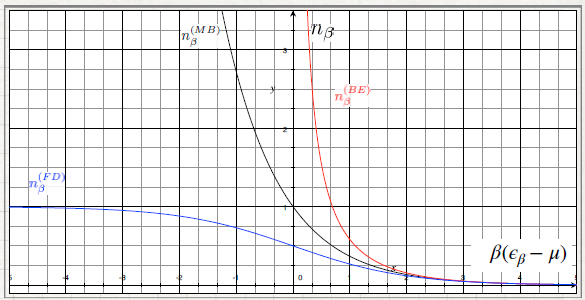
\includegraphics[width = \textwidth]{distributions.png}
    \caption{Maxwell-Boltzmann, Fermi-Dirac and Bose-Einstein distributions. We can see that for high temperature (on the right of the graph), the distributions converges. (in the figure the subscript $_k$ is instead denoted with $_\beta$)}
    \label{fig:distributions}
\end{figure}

Now that we got $ n_k$, we can also get the number of particles $N$, simply by evaluating:
\begin{equation}\label{eq:N}
    N = \sum_k \angles{\hat n_k} = \sum_k \frac1{e^{\beta(\epsilon_k-\mu)}\mp 1}
\end{equation} 
Or also, $N$ can also be obtained from:
$$ N = -\der{\Omega_{B/F}}\mu = (\ref{eq:N}) \text{ as exercise}$$

We can also evaluate the energy as:
$$ E = \sum_k \epsilon_k n_k = \sum_k \frac{\epsilon_k}{e^{\beta(\epsilon_k - \mu)} \mp 1}$$

\underline{\textbf{Thermodynamic limit}}\\
What we've done up to now works within a finite volume and in a discrete case:
$$ \epsilon_\alpha = \frac{\hbar^2\vec k^2}{2m} \qquad \text{periodic BCs} \to \vec k = \frac{2\pi}L(n_x,n_y,n_z) \qquad n_j \in \mathbb Z \qquad \alpha = (n_x,n_y,n_z)$$

In the thermodynamic limit $V,L \to \infty$, $\frac{2\pi}L \to 0$, so the space between different levels becomes smaller and smaller and $k$ becomes continuous. All the sum expressions become integrals. Let's see how. For a single component $n_j = n_x, n_y, n_z$:
\begin{align*}
    \sum_{n_j}() &= \sum_{n_j}()\underbrace{\Delta n_j}_{=1} &k_j = \frac{2\pi}L n_j \iff \Delta k_j = \frac{2\pi}L \Delta n_j\\
    &= \sum_{k_j}() \frac L{2\pi} \Delta k_j  &\Delta k_j \to dk_j \text{ in the limit}\\
    &= \frac L{2\pi} \int_{-\infty}^{\infty} dk_j ()    
\end{align*}
Repeating this procedure for all the components give us:
\begin{align*}
\sum_\alpha () = \sum_{n_x,n_y,n_z} () \to& \left(\frac L{2\pi}\right)^3 \int d^3k\ () = \frac V{(2\pi)^3} \int d^3 k \ ()
\intertext{Since sometimes we have $|\vec k|$, it is convenient to use spherical coordinates:}
&=\frac{V4\pi}{(2\pi)^3} \int_0^\infty k^2 dk\ f(|\vec k| = k) 
\intertext{since $\epsilon_\alpha = \epsilon_\alpha(k) = \frac{\hbar^2 k^2}{2m}$, we can change variable: $d\epsilon = \frac{\hbar^2 k}m dk$ }
&\stackrel{\text{as exercise}}{=} \frac V{2\pi^2}\left(\frac{2m}{\hbar^2}\right)^{3/2} \int_0^\infty \epsilon^{1/2} d\epsilon
\end{align*}
So: $$\sum_\alpha \to VA\int_0^\infty \epsilon^{1/2} d\epsilon \qquad \text{with } A = \frac 1{2\pi^2} \left(\frac{2m}{\hbar^2}\right)^{3/2}$$
we call $g(\epsilon) = A\epsilon^{\frac 12}$ \textbf{density of states}.
    
\gray{Since we are using $\epsilon_\alpha = \frac{\hbar^2k^2}{2m}$, this only works for non-interacting (free) non-relativistic particles. Also, we are assuming that we are in a three-dimensional space, otherwise the change of variable would be different.}

\begin{quote}
    Also notice something: in writing the grancanonical partition function (\ref{eq:grancanonical}), we didn't consider the fact that an energy level can be degenerate. If we want to take that into account, we would have:
    $$ \mathcal Z_{B/F} = \prod_\alpha \left[1 \mp e^{-\beta(\epsilon_\alpha - \mu)}\right]^{\mp g} $$
    $$ \Omega = \frac 1\beta \log \mathcal{Z} = \mp g\sum_\alpha \log\left[1 \mp e^{-\beta(\epsilon_\alpha - \mu)}\right]$$
    $$\text{and:}\qquad  N = g\sum\alpha\angles {\hat n_\alpha} \qquad E = g \sum_\alpha\epsilon_\alpha n_\alpha \qquad \text{etc}$$
\end{quote}

Now that we are in the continuous case, we can evaluate $\Omega, N, E$ as integrals. 
$$ \Omega = \pm V\frac A\beta \int_0^\infty \epsilon^{1/2}\log \left[1 \mp e^{-\beta(\epsilon_\alpha - \mu)}\right]d\epsilon $$
\begin{equation}\label{eq:N-withA}
    N = AV\int_0^\infty \epsilon^{1/2}\frac1{e^{\beta(\epsilon - \mu)} \mp 1}d\epsilon
\end{equation}
\begin{equation}\label{eq:E-withA}
    E = AV\int_0^\infty \epsilon^{3/2}\frac1{e^{\beta(\epsilon - \mu)} \mp 1}d\epsilon
\end{equation}
Notice that their expressions scale with $V$ (as it should be, since they are extensive quantities)

Integrating by parts:
\begin{align*}
    \frac{\Omega}V &= \frac A\beta \left\{\cancel{\left[\pm \frac23 \epsilon^{3/2} \log(\dots)\right]_0^\infty} \mp \int_0^\infty \frac23 \epsilon^{3/2} \frac{\pm \beta}{e^{\beta(\epsilon-\mu)}\mp 1}d\epsilon\right\}\\
    &= \frac23 A \int_0^\infty \epsilon^{3/2} \frac1{e^{\beta(\epsilon-\mu)}\mp 1}d\epsilon
\end{align*}
$$ \implies \underbrace{\Omega}_{-pV} = -\frac23 E \implies \boxed{pV = \frac23 E} \quad \text{Equation of state}$$
This is the equation of state of a perfect (quantum) gas. In the classical case, $E = \frac32 Nk_BT \implies pV = Nk_BT$

\subsection{Fundamental equations}
We can also calculate (remind that (-)Bosonic gas   (+)Fermionic gas):
$$ n = \frac NV = A\int_0^\infty \frac{\epsilon^{1/2}d\epsilon}{e^{\beta(\epsilon-\mu)}\mp 1} \qquad p = \frac23 \frac EV = \frac23 A \int_0^\infty \frac{\epsilon^{1/2}d\epsilon}{e^{\beta(\epsilon-\mu)}\mp 1}$$

By solving these equation, we would know the state of the gas (bosonic or fermionic). The problem is that they don't have a solution/primitive in 3D. We'll see the solution for low and high temperatures.\\
Using the fugacity $z = e^{\beta \epsilon}$:
\begin{align*}
n &= A\int_0^\infty \frac{\epsilon^{1/2}d\epsilon}{e^{\beta\epsilon}z^{-1} \mp 1}\\
&= A\int_0^\infty \frac{z\epsilon^{1/2}d\epsilon}{e^{\beta\epsilon}\mp z} = &\text{change of variable: $\beta\epsilon = x^2 \quad \beta d\epsilon = 2xdx$}\\
&= \frac{4g}{\sqrt\pi}\frac1{\lambda_T^3}\int_0^\infty \frac{zx^2dx}{e^{x^2}\mp z}
\end{align*}
with $\lambda_T = \frac \hbar{\sqrt{2\pi mk_BT}}$

Clearly, since we are not able to do the first integral, we can't do the last either, but:
$$ \frac{z}{e^{x^2}\mp z} = \frac{ze^{-x^2}}{1\pm ze^{-x^2}} = ze^{-x^2} \sum_{n=0}^\infty(\mp 1)^n \left(ze^{-x^2}\right)^n \quad \text{if the series is convergent}$$
For fermions(-), it converges $\forall z \notin \left[-\infty, -1\right]$\\
For bosons(+), it converges only for $z < 1 \implies \mu < 0$, but this is only what we needed to suppose from the beginning.
So $n$ becomes:
\begin{align*}
    n &= \frac{4g}{\sqrt \pi} \frac 1{\lambda_T^3} \int_0^\infty dx\ x^2 e^{-x^2}z \sum_{n=0}^\infty (\pm 1)^n \left(ze^{-x^2}\right)^n
    \intertext{and if the series is convergent I can swap the sum with the integral.}
    &= \frac{4g}{\sqrt \pi} \frac 1{\lambda_T^3} \sum_{n=0}^\infty (\pm 1)^n z^{n+1}\int_0^\infty dx\ x^2 e^{-(n+1)x^2}
\end{align*}
Now the integral can be evaluated, because it is the second moment of the Gaussian integral: $\frac{\sqrt \pi}4 \frac 1{(n+1)^{3/2}}$
$$ n= \frac g{\lambda_T^3} \sum_{n=0}^\infty \frac{z^{n+1}(\pm 1)^n}{(n+1)^{3/2}}$$

Similar calculations can be done for $p$, with the only difference being a $x^4$ instead of $x^2$ inside the integral. Thus obtaining:
$$p = k_BT \frac g{\lambda_T^3} \sum_{n=0}^\infty \frac{z^{n+1}(\pm 1)^n}{(n+1)^{5/2}}$$

If we define 
$$\text{Bosons} \qquad b_l(z) \equiv \sum_{n=0}^\infty \frac{z^{n+1}}{(n+1)^l}$$
$$\text{Fermions} \qquad f_l(z) \equiv \sum_{n=0}^\infty(-1)^n \frac{z^{n+1}}{(n+1)^l}$$
then we obtain the \textbf{fundamental equations}:
\begin{equation}\label{eq:fundamental}
    \boxed{n = \frac NV = \frac g{\lambda_T^3} \begin{cases} b_{3/2} (z) \\ f_{3/2}(z) \end{cases}
    \qquad \frac p {k_BT} = \frac g{\lambda_T^3} \begin{cases} b_{5/2}(z) \\ f_{5/2}(z) \end{cases}}
\end{equation}

In the classical limit $z \ll 1$, we can take just the first term of the $f_l$ and $g_l$ functions: $b_l(z) \simeq f_l(z) \simeq z$ so we get:
$$ n = \frac g{\lambda_T^3} z \implies z = \frac {n\lambda_T^3} g \ll 1 \quad \text{dilute gas, $\lambda_T^3$ small $\to T$ large}$$
$$ \frac{p}{k_BT} = \frac g{\lambda_T^3} z = n = \frac NV \implies pV = Nk_BT$$
which is the equation of a perfect classical gas, which we obtained from Bosons and Fermions statistic.

Also, in the limit of high temperatures we get the exact formulas for $\mu$ and $n(\epsilon)$ that we got for a classical gas:
$$ n = \frac g{\lambda_T^3} e^{\beta\mu} \implies \mu(T) = -\frac 32 k_BT \log\left(\frac {nk_BT}{2\pi\hbar^2 n^{3/2}}\right) \xrightarrow[T\to\infty]{} -\infty
$$
$$ \beta\mu \to -\infty \implies n(\epsilon) = \frac 1{e^{\beta(\epsilon-\mu)}\mp 1} \simeq e^{-\beta(\epsilon-\mu)} = n_{MB}$$
So in the limit of high temperatures, both the Bose-Einstein and the Fermi-Dirac distributions converges to the Maxwell-Boltzmann distribution.

\subsection{Semi-classical limit (exercise 2.1)}
\notedate{01/12/2022}
At first, we can study the semi-classical limit, by taking the expansion of the fundamental equations (\ref{eq:fundamental}):
$$\begin{cases}
    n= \frac g{\lambda_T^3}\left[z \pm \frac{z^2}{2^{3/2}}\right] &\text{(I)}\\
    \frac p{k_BT} = \frac g{\lambda_T^3}\left[z \pm \frac{z^2}{2^{5/2}}\right] &\text{(II)}
\end{cases}$$
We will derive $z = z(n)$ from the first and plug into the second equation:
$$ \text{from (I)} \quad \frac {z^2}{2\sqrt 2} \pm z \mp \frac{n\lambda_T^3}g = 0 $$
\begin{align*}
    \implies z_{1,2} &= \sqrt 2\left[^{(B)}_{(F)}\mp 1\pm^{(z_2)}_{(z_1)} \sqrt{1\pm \frac 2{\sqrt 2}\left(\frac{n\lambda_T^3}g\right)}\right]
    \intertext{If we expand up to second order: $\sqrt{1\pm x} \simeq 1 \pm \frac12x - \frac18 x^2$}
    &\cong \sqrt2\left[\mp 1\pm \left(1\pm \frac1{\sqrt2}\left(\frac{n\lambda_T^3}g\right) - \frac 14 \left(\frac{n\lambda_T^3}g\right)^2\right)\right]
\end{align*}
Now, which one between $z_1$ and $z_2$ should we accept? The one that made the $\mp1$ cancels with $\pm1$, since we already know that the first order of $z$ is $z\sim \frac{n\lambda_T^3}g$. So:
$$ z = \frac{n\lambda_T^3}g \mp \frac 1{2\sqrt2}\left(\frac {n\lambda_T^3}g\right)^2$$
Plugging this into (II) keeping only the first order of $\frac{n\lambda_T^3}g$, gives:
$$ \frac p{k_BT} = \frac g{\lambda_T^3} \frac{n\lambda_T^3}g\left[1\mp \frac1{4\sqrt2}\left(\frac{n\lambda_T^3}g\right)\right] = n\left[1 \mp \frac 1{2^{5/2}} \frac{n\lambda_T^3}g\right]$$
The term $\frac 1{2^{5/2}} \frac{n\lambda_T^3}g$ is called \textit{quantum correction} or \textit{semiclassical correction}.\\

We can notice the sign of the quantum correction: it is - for bosons and + for fermions. That means that the pressure $p$ is reduced by bosonic gases and increased by fermionic gases, as if there is an attractive potential between bosons and a repulsive between fermions.\\
We also notice that the correction is quantum in nature, as it is shown by the fact that it goes to zero when $h \to 0 \implies \lambda = \frac h{\sqrt{2m k_BT}} \to 0 $ or when $g = 2S +1 \to \infty$, i.e. when all states have an infinite degeneracy so that quantum counting does not have anymore effect.\\

How much high should the temperature $T$ be to have $z \ll 1$? It depends on $n$: it must be \quad $n\lambda_T^3 \ll 1$.\\

Now let's do the opposite limit and analyze very low temperatures:

\subsection{Fermions at T=0}
Starting from the Fermi-Dirac distribution:
$$n_\alpha = \frac 1{e^{\beta(\epsilon_\alpha -\mu)} +1}$$
we'll take the limit $T\to 0 \implies \beta \to \infty$, so the behaviour of $n_\alpha$ depends on the sign of $\epsilon-\mu$:
\begin{itemize}
    \item if $\epsilon_\alpha -\mu < 0 \implies \epsilon_\alpha < \mu \implies n_\alpha \xrightarrow[\beta\to\infty]{}1 \quad \forall \epsilon_\alpha$
    \item if $\epsilon_\alpha -\mu > 0 \implies \epsilon_\alpha > \mu \implies n_\alpha \xrightarrow[\beta\to\infty]{}0 \quad \forall \epsilon_\alpha$
    \item if $\epsilon_\alpha -\mu = 0 \implies \epsilon_\alpha = \mu \implies n_\alpha =\frac12$
\end{itemize}

We call the \textbf{Fermi energy}: $\boxed{\epsilon_F \equiv \lim_{T\to 0}\mu(T)}$\\
So at $T=0$, the Fermi distribution is a step function: all states with energy $\epsilon <\epsilon_F$ are occupied (with only 1 particles, since they are fermions) and all the states with energy $\epsilon > \epsilon_F$ are empty (red in Fig. \ref{fig:fermions})

\begin{figure}[ht]
    \centering
    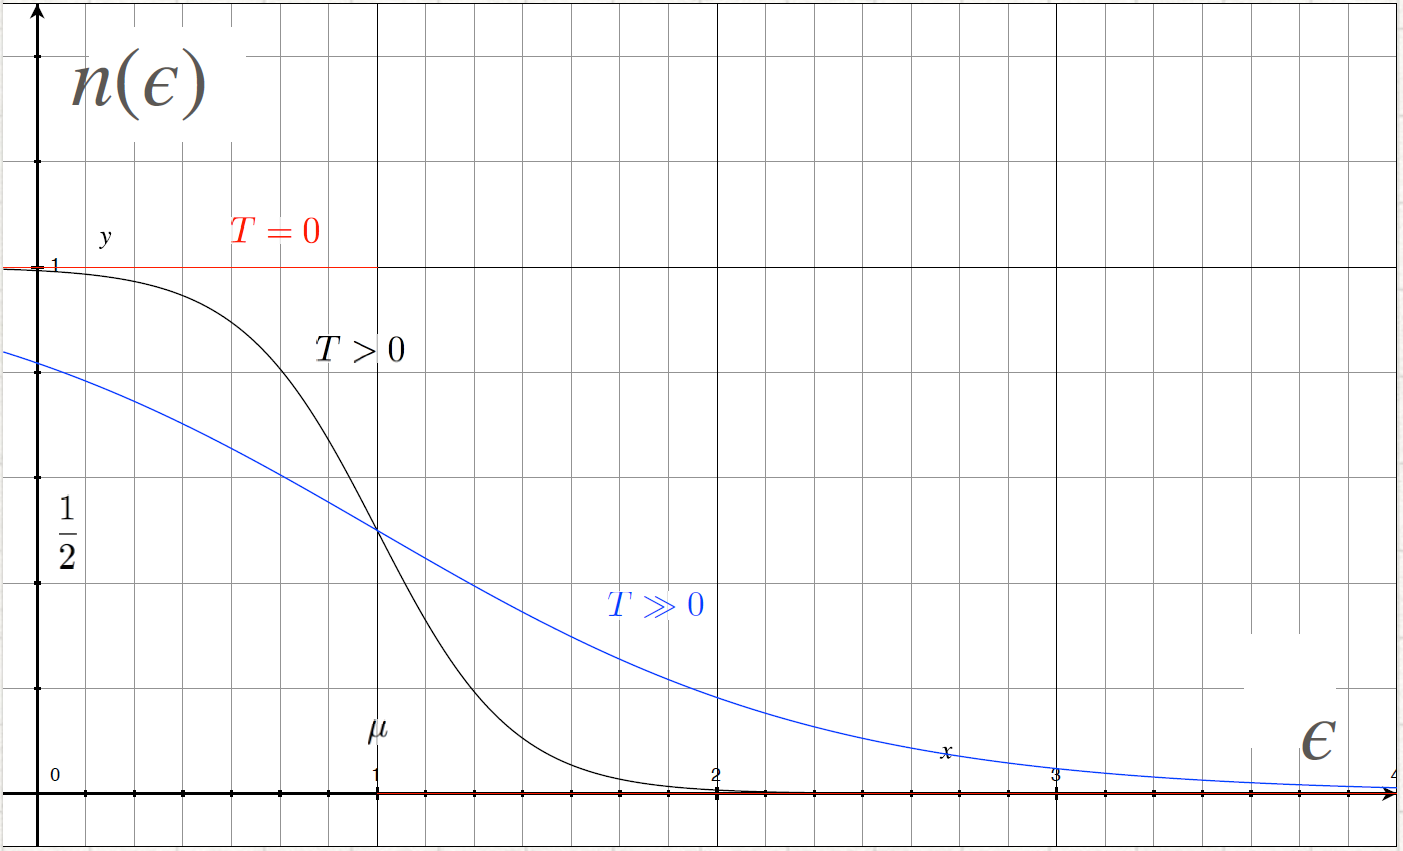
\includegraphics[width = \textwidth]{fermions.png}
    \caption{Fermions distribution at different temperatures}
    \label{fig:fermions}
\end{figure}

$\epsilon_F$ is defined by the number of particle $N$ (since there is just one particle for every $\epsilon_\alpha$), so the equation $N = \sum_\alpha n_\alpha$ fixes $\mu(T)$. In other words, to change the Fermi energy we have to change the number of particles.\\
\gray{Now $z = e^{\beta\mu}$ is no longer small.\\
Also recall that any $f_l(z)$ is convergent $\forall z <1$ and it's a smooth function.}

We can also define the \textbf{Fermi temperature} as: $\epsilon_F = k_B T_F$. If a system has a temperature $T \ll T_F$, then we are in the so-called \textbf{degeneration limit} and the system behaves effectively as at $T=0$ ($n(\epsilon)$ actually look like a step function and the calculations are easier). Examples could be:
\begin{itemize}
    \item conduction electrons in metals, with $T \sim 100K $ and $T_F \sim 10^4 - 10^5 K$
    \item free electrons in white dwarfs (ionised helium), with $T \sim 10^7 K$ and $T_F \sim 10^{11}$ since the density is very high ($n \sim 10^{30}/cm^3$)\\ \gray{(even if, at this temperature, speeds are relativistic --we will see later)}
\end{itemize}
The initial equations (\ref{eq:N-withA}) and (\ref{eq:E-withA}), becomes for $T=0$:
$$\frac NV = gA\int_0^\infty d\epsilon \frac{\epsilon^{1/2}}{e^{\beta(\epsilon-\mu)}+1} \stackrel{(*)}= gA \int_0^{\epsilon_F} d\epsilon\ \epsilon^{1/2} = gA\frac23\epsilon_F^{3/2}$$
$$\frac EV = gA\int_0^\infty d\epsilon \frac{\epsilon^{3/2}}{e^{\beta(\epsilon-\mu)} +1} \stackrel{(*)}= gA\int_0^{\epsilon_F} d\epsilon\ \epsilon^{3/2} = gA\frac25\epsilon_F^{5/2} $$
$(*)$ is justified because, when $T=0 \quad \frac 1{e^{\beta(\epsilon-\mu)}+1} = n_\alpha \ne 0 \ (=1)$ only if $\epsilon < \epsilon_F$.

\begin{comment}
and since we know that $\frac 1{e^{\beta(\epsilon-\mu)}+1} = n_\alpha \xrightarrow[\beta \to \infty]{} 1,0,\frac12$:
$$ n = gA\int_0^{\epsilon_F} d\epsilon \ \epsilon^{1/2} = gA \frac 23 \epsilon_F^{3/2}\implies \epsilon_F = \frac 3{2gA} n^{2/3}$$
Also, for a non-relativistic gas $\epsilon_F = {\hbar^2}{2m}k_F^2$ and we call $\hbar k_F$ the \textbf{Fermi momentum}.

%A = \frac 1{2\pi^2} \left(\frac{2m}{\hbar^2}\right)^{3/2}

\vspace{10pt}
Going back to calculations, we can also obtain the temperature:
$$\frac32 p = \frac EV = gA\int_0^\infty d\epsilon \frac{\epsilon^{1/2}\epsilon}{e^{\beta(\epsilon-\mu)} +1} \stackrel{T=0}= gA\int_0^{\epsilon_F} d\epsilon\ \epsilon^{3/2} = gA \frac 25\epsilon_F^{5/2}$$
\end{comment}

From the first expression, one gets: $\epsilon_F = \left(\frac32 \frac n {gA}\right)^{2/3}$ and dividing the second by the first, we can get the energy for particle: $\frac EV = \frac35 \epsilon_F$.
Using this and the fact that $-pV = \Omega = -\frac23 E\ $ we can get: $$p= \frac25\frac NV \epsilon_F = \frac23 n \epsilon_F$$ 
So notice that at $T=0$, \quad $p > 0$.\\ This is a consequence of the Pauli exclusion principle\\
\gray{Remark: it is also possible to expand the fundamental equations for small temperatures, using the Sommerfield expansion.}

\subsection{Bosons at T=0}
\notedate{(XI) MON 05/12/2022}
We will start from the fundamental equation (\ref{eq:fundamental}) for bosons, recalling that the series $b_{3/2}(z)$ it's only convergent if $|z| < 1$. At $z=1$,  $g_{3/2}(z)$ is still defined and it's called the Reimann function $\zeta(3/2)$, but it has a vertical derivative ($g'_{3/2}(1) = \infty$), so the function is no longer analytic. This is a signal that something is happening in the gas of bosons. Since, $z = e^{\beta\mu}$, let's focus on the chemical potential $\mu(T)$.

\begin{itemize}
    \item We proved that in the classical limit, $\mu(T) \xrightarrow[T\to\infty]{}-\infty$
    \item From general thermodynamics it can be proved that: $\der\mu T \le 0$ \item For bosons, we proved that $\mu \le 0$ (from the definition of $\Z$). 
\end{itemize}
So there are only two possibilities:
\begin{enumerate}
    \item $\mu(T)\to 0$ for $T\to 0$, which is what happen for a non-relativistic Bose gas in 2D (Fig. \ref{fig:mu(T)} left).
    \item $\mu(T) \to 0$ for finite $T_c > 0$, which is what we have for a non-relativistic Bose gas in 3D (Fig. \ref{fig:mu(T)} right)
\end{enumerate}

\begin{figure}[ht]
    \centering
    \begin{subfigure}[b]{0.48\textwidth}
        \centering
        \begin{tikzpicture}
            \draw[->](0,2.5) -- (5.5,2.5) node[anchor=west] {$T$};
            \draw[->](0.5,0) -- (0.5,3.5) node[anchor=east] {$\mu$};
            \draw(0.5,2.5) parabola (5,0.5);
        \end{tikzpicture}
    \end{subfigure}
    \begin{subfigure}[b]{0.48\textwidth}
        \centering
        \begin{tikzpicture}
            \draw[->](0,2.5) -- (7,2.5) node[anchor=west] {$T$};
            \draw[->](0.5,0) -- (0.5,3.5) node[anchor=east] {$\mu$};
            \draw(2,2.5) parabola (7,0.5);
            \fill (2,2.5) circle (0.07cm) node[anchor=north] {$T_c$};
        \end{tikzpicture}
    \end{subfigure}
    \caption{$\mu(T)$ for 2D (left) and 3D non-relativistic Bose gas}
    \label{fig:mu(T)}
\end{figure}

Now we would like to find $T_c$. We can invert the first fundamental equation (\ref{eq:fundamental}) to get $\mu(T)$:
$$\text{from} \quad n = \frac g{\lambda_T^3} g_{3/2}(z) \to \mu = \mu(T)$$
$T_c$ will be the (critical) temperature such that: $\mu(T=T_c) = 0$ and we can find it by evaluating $n$ with $z=1$ (since $z=e^{\beta\mu}$):
$$ n = \frac g{\lambda_T^3} g_{3/2}(z=1) \xrightarrow[T\to 0]{} 0$$
This is absurd: particles are not leaving the container! There must be something we have missed and this formula is not correct in the range $T < T_c$.

To understand why, let's go back to the Bose-Einstein distribution:
$$n_{BE}(\epsilon) = \frac1{e^{\beta(\epsilon-\mu)}-1} \stackrel{\mu=0}= \frac 1{e^{\beta\epsilon}-1}$$ 
which is well defined if $\epsilon > 0$, but divergent if $\epsilon =0$:
$$n_{BE}(\epsilon = 0) = \lim_{\epsilon\to 0}\frac1{e^{\beta\epsilon}-1} \to \infty$$ 
So the $\epsilon = 0$ level is filled with an increasing number of particles. In other words, particles like to go in the ground state.

So the number of particles in the $\epsilon =0$ state diverges: $N_0 \equiv N_{\epsilon=0} = \infty$.
That means that, even if in the thermodynamic limit $N\to \infty$, the ratio $\frac {N_0}N$ stays finite, while usually $\frac{N(\epsilon\ne 0)}N$ is infinitesimal and such that $\int_0^\infty \frac{N(\epsilon\ne0)}N d\epsilon = 1$.\\
This is what we call \textit{macroscopic occupation} of the ground state.\\
We can also define the density of particle in the ground state (\textbf{ground state density}) as: 
$$n_0\equiv \frac{N_0}V = \frac{N_0}N\frac NV = \frac{N_0}N n$$
which is finite.

We can now notice something: $n = \frac g{\lambda_T^3} g_{3/2}$ is the TD limit of the equation:
$$ N = \sum_\alpha n_{BE}(\epsilon_\alpha) = \sum_\epsilon \frac 1{e^{\beta(\epsilon-\mu)}-1} \xrightarrow[\text{TD limit}]{}V\int_0^{\infty} d\epsilon \ g(\epsilon) n_{BE}(\epsilon)$$
$\epsilon =0 $ is just an external point of the integral $\int_0 d\epsilon \dots$, so even if $n_{BE}\xrightarrow[]{\epsilon\to 0}\infty$, the integral is convergent. That is the reason why we didn't see the divergence when we performed the calculations. But now, if $\mu= 0$, then the fraction of particles in $\epsilon = 0$ becomes macroscopic and, as we have seen, it gives problems if we don't consider it, so we have to add it manually, writing:
\begin{align*} N = &\sum_\epsilon n_{BE} (\epsilon) = n_{BE}(0) + \sum_{\epsilon > 0}n_{BE}(\epsilon)  = N_0 + \sum_{\epsilon>0}n_{BE}(\epsilon)\\
\xrightarrow[\text{TD limit}]{} &\ N_0 + V\int_0^{\infty} d\epsilon \ g(\epsilon) n_{BE}(\epsilon) \end{align*}
and the integral is not divergent since $n(\epsilon\ne0)$ in 0 is infinitesimal.

Dividing by $V$ we obtain:
$$n = n_0 + \frac g{\lambda_T^3} g_{3/2}(z) = n_0 + n_n(T) \qquad n_{normal} \equiv n(\epsilon \ne 0)$$
\begin{itemize}
    \item for $T\ge T_c \qquad n_0 = \frac{N_0}V\xrightarrow[\text{TD limit}]{}0  \qquad n_n(T)= n = \frac g{\lambda_T^3} g_{3/2}(z)$ 
    \item for $T\le T_c \qquad \qquad n_0(T) = n-n_n \ne 0 \qquad n_n = \frac g{\lambda_T^3} g_{3/2}(1) = \frac g{\lambda_T^3}\frac{n\lambda_{T_c}^3}g = \left(\frac T{T_c}\right)^{3/2} n$ 
\end{itemize}

So:
$$
    n_0(T) = \begin{cases} 0 & T \ge T_c \\ n\left[1- \left(\frac T{T_c}\right)^{3/2}\right] & T < T_c \end{cases} \qquad 
    n_n(T) = \begin{cases} n & T \ge T_c \\ n\left(\frac T{T_c}\right)^{3/2} & T < T_c \end{cases}
$$
As you can notice in Fig. \ref{fig:n0-nn}, both $n_0(T)$ and $n_n(T)$ are continuous at $T=T_c$ but not differentiable. As always happen, this is the sign of a \textbf{phase transition}: in this case between a quantum gas to a Bose-Einstein condensate. This is a new state of matter, so the population of the ground state actually has a macroscopic effect.

\begin{figure}[ht]
    \centering
    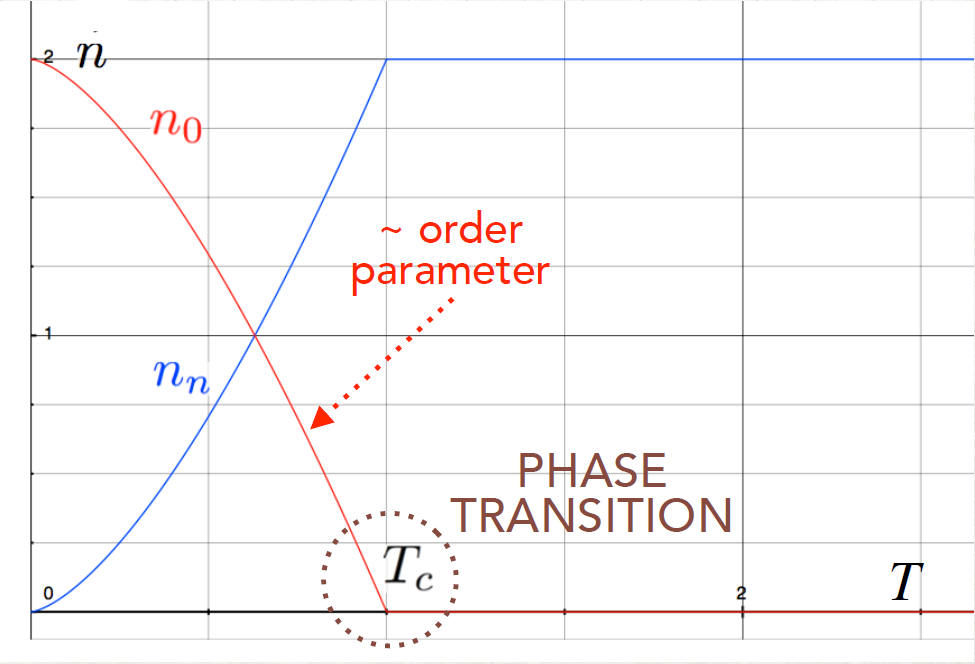
\includegraphics[width = 8cm]{images/n0 and nn.png}
    \caption{$n_n(T)$ and $n_0(T)$. For $T < T_c$ we have a Bose-Einstein condensate.}
    \label{fig:n0-nn}
\end{figure}

We could analyze the other fundamental equation (\ref{eq:fundamental}), to see that is has no problems $\forall z$ and $\forall T$, because $g_{5/2}$ doesn't have the same divergence problem as $g_{3/2}$:
$$
    \frac p{k_BT} = \frac g{\lambda_T^3} g_{5/2}(z) \qquad \text{both with } \begin{cases}
        z= e^{\beta\mu} & T\ge T_c\\ z=1 & T \le T_c
    \end{cases} 
$$
%\vspace{20pt}

\underline{\textbf{Thermodynamical quantities}}
\begin{itemize}
    \item Energy per particle $u(T) = \frac EV$\\
    Using the above equations and recalling that:
    $$-pV = \Omega = -\frac23 E \quad \implies \quad \frac EV = \frac32p = \frac32 k_BT \frac p{k_BT} = \frac32 k_BT \frac g{\lambda_T^3} g_{5/2}(z)$$
    we can calculate 
    \begin{align*}
        u &\equiv \frac EN = \frac {E/V}{N/V} = \frac{E/V}{n(T)} \\
        &= \frac{3k_BT}2 \begin{cases} 
            \frac{g_{5/2}(z)}{g_{3/2}(z)} & T \ge T_c \\ 
            \frac{g_{5/2}(1)}{g_{3/2}(1)} \left(\frac T{T_c}\right)^{3/2} & T \le T_c \end{cases}
    \end{align*}
    which is continuous at $T = T_c$.

    \item Specific heat (at constant $V$) per particle $c_V = \left.\der uT\right|_V = \left.\frac1N\der ET\right|_V = \frac {C_V}N$\\
    This is a really complex calculation for $T\ge T_c$.\\
    Recall that classically we had $E = N \frac32 k_BT$, so $c_V = \frac32 k_BT$, which was wrong for low temperatures ($c_V\xrightarrow[T\to 0]{}0$ classically). Now quantum mechanics solves the problem and we can correct it. $c_V(T)$ is plotted in Fig. \ref{fig:cv}, where we can see that it is continuous in $T_c$ but not differentiable (it has a cusp). This is again another signal of a phase transition.
    \begin{figure}[ht]
        \centering
        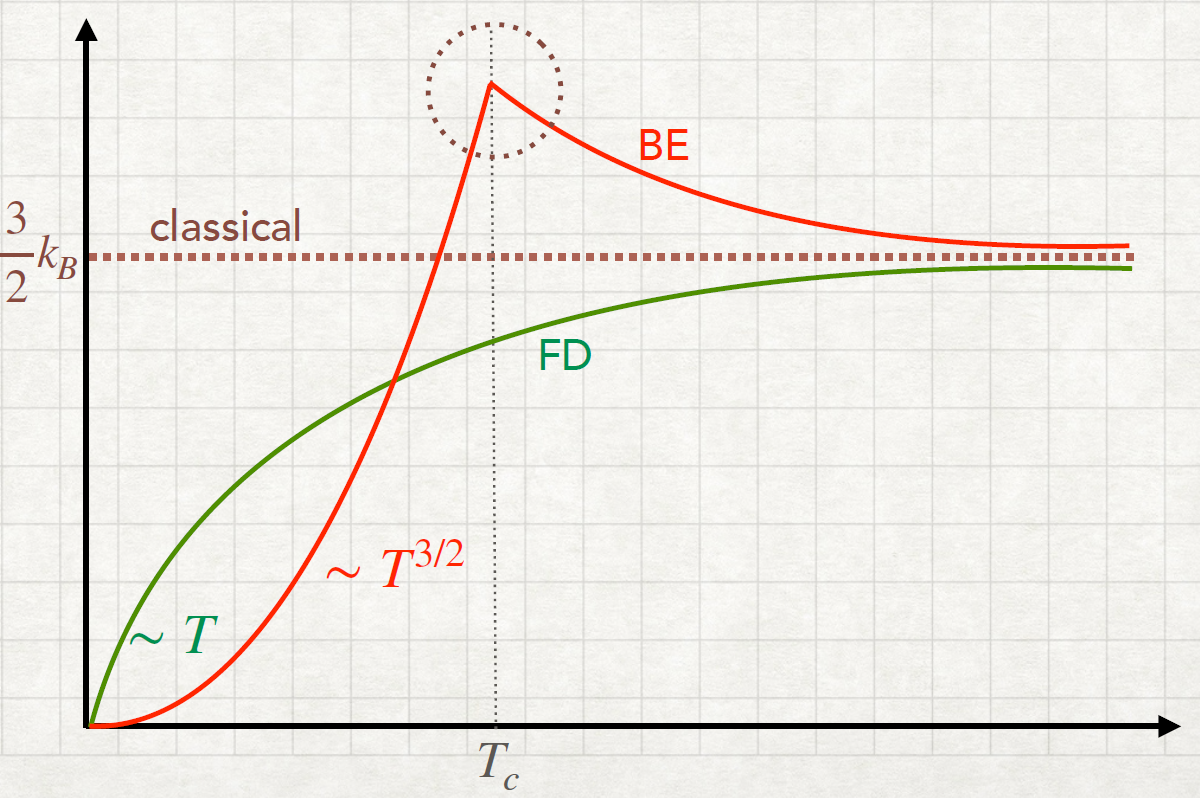
\includegraphics[width = 8cm]{images/cv(T).png}
        \caption{$c_V(T)$ for Bosons (red) and Fermions (green). In the Bose-Einstein distribution, the cusp at $T_c$ indicate a phase transition.}
        \label{fig:cv}
    \end{figure}

    \item Entropy $S$\\
    $$
        S = \frac{E-\Omega -\mu N}T = 
        k_B\left(\frac{E+\frac23 E-N\beta^{-1}\log Z}{k_BT}\right) =
        k_BN\left(\frac53\frac1{k_BT}\frac EN -\log Z\right)
    $$
    Since $z = e^{\beta\mu}\qquad -pV= \Omega = -\frac23 E$.

    \begin{align*}
        s &= \frac SN = k_B\left[\frac53\frac{E/N}{k_BT} - \log z\right]\\
        &= k_B\left(\frac52\frac{g_{5/2}(z)}{g_{3/2}(z)} - \frac{g_{3/2}(z)}{g_{3/2}(z)}\log z\right)\\
        &= \frac {k_B}{g_{3/2}(z)}\left[\frac52g_{5/2}(z) - g_{3/2}(z)\log z\right]\\
        &= \frac{k_B}{g_{3/2}} \left(\frac T{T_c}\right)^{3/2}\left(\frac52g_{5/2}(z) - g_{3/2}(z)\log z\right)
    \end{align*}
    We can check that this equation holds $\forall T$ as long as we use $g_l(z) = g_l(1)$ for $T \le T_c$:
    \begin{itemize}
        \item $T>T_c \qquad z<1\qquad$ all good
        \item $T=T_c \qquad s(T=T_c) = \frac52 k_B\frac{g_{5/2}(1)}{g_{3/2}(1)}$
        \item $T<T_c \qquad s = \frac52 k_B\left(\frac T{T_c}\right)^{3/2}\frac{g_{5/2}(1)}{g_{3/2}(1)} \xrightarrow[T\to 0]{}0$\\
        however, at $T=0$, all the particles are in the ground state ($n_0(T) \xrightarrow[T\to0]{}n$. This means that particles in the condensate carry no entropy $S_{cond} = 0$. So $s$ below $T_c$ gets smaller and smaller as $T$ decreases, since more and more particles go to the ground state.
    \end{itemize}
        
    Consider one particle jumping from $\epsilon > 0$ to the ground state at $T=T_c$. Then:
    $$ \Delta s = s(T=T_c) - 0 = k_B\frac 53 \frac{g_{5/2}(1)}{g_{3/2}(1)} \ne 0$$
    But we also know that $0 \ne \Delta S = \Delta Q / T_c$. So the process of of decaying from $\epsilon > 0$ to $\epsilon =0$ costs some energy, some heat. This heat $\Delta Q \ne 0$ is called latent heat.

    This is a peculiar phase transition, with continuous thermodynamic potentials, but latent heat as (for instance) in evaporation.

    \gray{It is the same as water boiling, which stops at $T= 100^oC$ since particles absorb latent heat.}
\end{itemize}

\notedate{(XII) MON (ex.3) 12/12/2022}
\notedate{(XIII) MON (ex.4) 19/12/2022}
\subsection{Exercise (2.5): Gas of photons}
Let us consider a gas of photons, confined in a volume $V$ at equilibrium at a temperature $T$.
Photons are ultra-relativistic bosonic particles, for which: $\epsilon_{\vec p} = c|\vec p|$. They can be absorbed/emitted so that their particle number is not conserved, providing an example of bosonic systems with zero chemical potential: $\mu(T) \equiv 0$. Recall also that photons have two independent polarizations, so that g = 2.
\begin{enumerate}
    \item \textbf{Density of states:}\\
    The density of states is easily obtained from $$\Sigma(\epsilon) = g\int_{cp < \epsilon} \frac{d^3 x\ d^3p}{h^3} = \frac{8\pi V}{h^3} \int_0^{\epsilon/c} dp \ p^2 = \frac{8\pi V}{3(hc)^3}\epsilon^3$$
    since $\omega (\epsilon) = \partial\Sigma / \partial \epsilon$.
    \item \textbf{Granpotential, number of particles, internal energy}\\
    From the previous point it follows that:
    $$\Omega = \frac 1\beta \int_0^\infty d\epsilon \ \omega(\epsilon) \log(1-e^{\beta \epsilon}) = -\frac{8\pi V}{3(hc)^3} \int_0^\infty \frac{\epsilon^3}{e^{\beta \epsilon} - 1} d\epsilon$$
    where the last equality has been found after integration by parts.\\Similarly, one gets:
    $$ N = \int_0^\infty d\epsilon \ \omega(\epsilon) n(\epsilon) = \frac{8\pi V}{(hc)^3} \int_0^\infty \frac{\epsilon^2}{e^{\beta \epsilon}-1} d\epsilon$$
    $$ E= \int_0^\infty d\epsilon \ \omega(\epsilon)\epsilon n(\epsilon) = \frac{8\pi V}{(hc)^3} \int_0^\infty\frac{\epsilon^3}{e^{\beta \epsilon}-1}d\epsilon$$
    From the relation $\Omega = -pV$ it follows that: $p = \frac 13 \frac EV$
    \item \textbf{Density of energy and particles}\\
    Using the relation 
    $$\int_0^\infty \frac{x^n}{e^x -1}dx = \zeta(n+1)$$
    we can show that:
    $$ \frac NV = \frac{8\pi \zeta(3)}{(hc)^3} (k_BT)^3$$
    $$ \frac EV = \frac{8\pi\zeta(4)}{(hc)^3}(k_BT)^4$$
    Also, as a consequence of $C_V = \partial E / \partial T$, we have: $c_v = \frac{C_V}V \propto T^3$
    \item \textbf{Spectral distribution and density}
    Recalling that the energy of a photon is related to the frequency through: $\epsilon = h\nu$, we can consider the number of photons $N(\nu)$ with an energy $0 \le \epsilon \le h\nu$, given by:
    $$ N(\nu) = \frac{8\pi V}{(hc)^3} \int_0^{hv} \frac{\epsilon^2}{e^{\beta \epsilon}-1}d\epsilon$$
    We can calculate the spectral distribution:
    $$f(\nu) = \frac{dN(\nu)}{d\nu} = \frac{8\pi V}{(\beta h c)^3}\frac{(\beta h \nu)^2}{e^{\beta h \nu}-1} \beta h = \frac{8\pi V}{c^3}\frac{v^2}{e^{\beta h v}-1}$$
    This represents the number of photons with frequency between $\nu$ and $\nu + d\nu$.
    We can also show that the energy spectral density (defined as the energy for unit frequency and volume) is:
    $$u(\nu) = \frac{8\pi h}{c^3} \frac{\nu^3}{e^{\beta h \nu}-1}$$
    \item \textbf{Wein's and Rayleigh-Jeans' laws}\\
    Rayleigh-Jeans' law is obtained by expanding the exponential function in the denominator at first order, while Wien's law is got by neglecting the addend -1 in the denominator:
    $$u(\nu) \simeq 8\pi h\left(\frac vc\right)^3 e^{-\beta h \nu} \qquad \beta h \nu \gg 1$$
    $$ u(\nu) \simeq \frac{8\pi h}{c^3} \frac{\nu^3}{\beta h \nu} = \frac{8\pi}{c^3\beta} \nu^2 \qquad \beta h \nu \ll 1$$
\end{enumerate}